%% 
%% Copyright 2007-2020 Elsevier Ltd
%% 
%% This file is part of the 'Elsarticle Bundle'.
%% ---------------------------------------------
%% 
%% It may be distributed under the conditions of the LaTeX Project Public
%% License, either version 1.2 of this license or (at your option) any
%% later version.  The latest version of this license is in
%%    http://www.latex-project.org/lppl.txt
%% and version 1.2 or later is part of all distributions of LaTeX
%% version 1999/12/01 or later.
%% 
%% The list of all files belonging to the 'Elsarticle Bundle' is
%% given in the file `manifest.txt'.
%% 
%% Template article for Elsevier's document class `elsarticle'
%% with harvard style bibliographic references

\documentclass[preprint,12pt,authoryear]{elsarticle}

%% Use the option review to obtain double line spacing
%% \documentclass[authoryear,preprint,review,12pt]{elsarticle}

%% Use the options 1p,twocolumn; 3p; 3p,twocolumn; 5p; or 5p,twocolumn
%% for a journal layout:
%% \documentclass[final,1p,times,authoryear]{elsarticle}
%% \documentclass[final,1p,times,twocolumn,authoryear]{elsarticle}
%% \documentclass[final,3p,times,authoryear]{elsarticle}
%% \documentclass[final,3p,times,twocolumn,authoryear]{elsarticle}
%% \documentclass[final,5p,times,authoryear]{elsarticle}
%% \documentclass[final,5p,times,twocolumn,authoryear]{elsarticle}

%% For including figures, graphicx.sty has been loaded in
%% elsarticle.cls. If you prefer to use the old commands
%% please give \usepackage{epsfig}
\usepackage{epsfig}

%% packages added
\usepackage{svg}
\usepackage{wasysym}
\usepackage{amsmath}
\usepackage{subcaption}
\usepackage{bm}

%% The amssymb package provides various useful mathematical symbols
\usepackage{amssymb}

\usepackage{nomencl} % Nomenclature package
\makenomenclature

%% This code creates the nomenclature
% -----------------------------------------
\usepackage{etoolbox}
\renewcommand\nomgroup[1]{%
  \item[\bfseries
  \ifstrequal{#1}{A}{Acronyms}{%
  \ifstrequal{#1}{G}{Greek symbols}{%
  \ifstrequal{#1}{R}{Roman symbols}{}}}%
]}
% -----------------------------------------

%% The amsthm package provides extended theorem environments
%% \usepackage{amsthm}

%% The lineno packages adds line numbers. Start line numbering with
%% \begin{linenumbers}, end it with \end{linenumbers}. Or switch it on
%% for the whole article with \linenumbers.
%% \usepackage{lineno}

\newcommand{\anu}[1]{{\color{red}{#1}}}
\newcommand{\dmm}[1]{{\color{blue}{#1}}}


\usepackage[hidelinks]{hyperref}

\journal{Combustion and Flame}

\begin{document}

\begin{frontmatter}

%% Title, authors and addresses

%% use the tnoteref command within \title for footnotes;
%% use the tnotetext command for theassociated footnote;
%% use the fnref command within \author or \affiliation for footnotes;
%% use the fntext command for theassociated footnote;
%% use the corref command within \author for corresponding author footnotes;
%% use the cortext command for theassociated footnote;
%% use the ead command for the email address,
%% and the form \ead[url] for the home page:
%% \title{Title\tnoteref{label1}}
%% \tnotetext[label1]{}
%% \author{Name\corref{cor1}\fnref{label2}}
%% \ead{email address}
%% \ead[url]{home page}
%% \fntext[label2]{}
%% \cortext[cor1]{}
%% \affiliation{organization={},
%%            addressline={}, 
%%            city={},
%%            postcode={}, 
%%            state={},
%%            country={}}
%% \fntext[label3]{}

%\title{Assessment of a multiregime flamelet model in partially-premixed laminar conditions \textbf{OR} Flame index partitioning for partially premixed combustion}

\title{Analysis of multiregime phenomena in a planar coflow flame using tabulated chemistry with a flame index}

%% use optional labels to link authors explicitly to addresses:
%% \author[label1,label2]{}
%% \affiliation[label1]{organization={},
%%             addressline={},
%%             city={},
%%             postcode={},
%%             state={},
%%             country={}}
%%
%% \affiliation[label2]{organization={},
%%             addressline={},
%%             city={},
%%             postcode={},
%%             state={},
%%             country={}}


% --------- Authors
\author[1]{Carlos Guillamón\corref{cor1}}
\cortext[cor1]{Corresponding author}
\ead{carlos.guillamon@bsc.es}

\author[1]{Anurag Surapaneni}
\author[2]{Arnaud Mura}
\author[3]{Enric Illana}
\author[1]{Daniel Mira}

%-------- Adresses/Affiliations
% Safran Tech
\affiliation[1]{organization={CASE Department, Barcelona Supercomputing Center},
            addressline={Plaça d'Eusebi Güell, 1}, 
            city={08034},
            country={Spain}}

% CERFACS
\affiliation[2]{organization={Institut PPRIME – UPR 3346, Université de Poitiers},
            addressline={ISAE-ENSMA and Université de Poitiers}, 
            %city={Toulouse},
            %citysep={}, % Uncomment if no comma needed between city and postcode
            %postcode={31057}, 
            city={??},
            country={France}}


% Coria
\affiliation[3]{organization={Department of Energy Plant Technology (LEAT)},
            addressline={Ruhr-University Bochum}, 
            %city={Saint-Etienne-du-Rouvray},
            %citysep={}, % Uncomment if no comma needed between city and postcode
            %postcode={76801}, 
            city={Bochum},
            country={Germany}}


%\affiliation{organization={},%Department and Organization
%            addressline={}, 
%            city={},
%            postcode={}, 
%            state={},
%            country={}}







\begin{abstract}
%% Text of abstract
\textbf{(Modify accordingly)})
Computations with combustion models based on flamelet libraries have been widely used in the past years due to their lower computational cost compared to detailed chemistry. Nevertheless, their main drawback is the need to precompute the flamelets either in fully premixed or non-premixed combustion modes, which might hinder the retrieval of partially-premixed characteristics such as those found in real system. Therefore, methods being able to account for such combination of modes in combustion simulations are needed. This paper presents an in-depth analysis of a flame index partitioning for distinguishing between premixed and diffusion modes. ...

\end{abstract}

%%%Graphical abstract
%\begin{graphicalabstract}
%%\includegraphics{grabs}
%\end{graphicalabstract}

%%Research highlights
% For inspiration, see 2023 Kuhn - A numerical study of ...
%\begin{highlights}
%\item Proposed injection methodology to learn boundary conditions from resolved atomization simulations
%\item New method to account for liquid dense core - gaseous turbulence interaction
%\item Parametric study of injection boundary conditions in dispersed phase computations.
%\end{highlights}

\begin{keyword}
%% keywords here, in the form: keyword \sep keyword

Partially premixed combustion  \sep non-premixed combustion \sep premixed combustion \sep flamelet methods \sep flame index \sep premixedness index \sep multi-regime flamelet model 



%% PACS codes here, in the form: \PACS code \sep code

%% MSC codes here, in the form: \MSC code \sep code
%% or \MSC[2008] code \sep code (2000 is the default)

\end{keyword}

\end{frontmatter}

%% \linenumbers

\clearpage


\printnomenclature


\nomenclature[A]{DC}{Detailed Chemistry}
\nomenclature[A]{FPI}{Flame-Prolongated ILDM}
\nomenclature[A]{FGM}{Flamelet Generated Manifold}
\nomenclature[A]{FPV}{Flamelet Progress Variable}
\nomenclature[A]{ILDM}{Intrinsic Low-Dimensional Manifold}
%\nomenclature[A]{\(TC\)}{Tabulated Chemistry}
\nomenclature[A]{TC}{Tabulated Chemistry}
\nomenclature[A]{TI}{Takeno Index}

\nomenclature[G]{$\xi$}{Flame index}



\nomenclature[R]{$C$}{Scaled progress varaible}
\nomenclature[R]{$Z$}{Mixture fraction}
\nomenclature[R]{$Y_c$}{Progress varaible}




\clearpage

%% main text
\section{Introduction}
\label{sec:intro}
%\input{01_intro}
%\clearpage

Accurate computations of reactive flows require a precise  description of chemical effects. For a reliable representation, Detailed Chemistry (DC) can be used for resolving the chemical reactions and transport equations for all species included in detailed mechanisms \citep{poinsot_theoretical_2005}. These methods present the advantage that no additional models are needed to obtain a complete description of chemistry. However, they require a high computational cost, since they need to resolve all chemical activity involving numerous chemical species, which in complex mechanisms can add up to hundreds of transport equations. Another family of methods are based on tabulated chemistry (TC), which are more attractive than DC from the point of view of computational resources. These methods rely on the precomputation of several 1D flames with detailed chemistry, and then mapping the resulting characteristics into a space based on reduced variables which are tabulated. The most widely used variables in the flamelets space are the mixture fraction $Z$ and the progress variable $Y_c$ \citep{janicka_calculation_1982}. Transport equations for these variables are solved during the computations, and transport and chemical properties (such as molecular weights, specific heats, and source terms) are then read from the tables. Accordingly, the number of transport equations to resolve is lower than in DC, resulting in significant computational savings. On the other hand, their main disadvantage is that the combustion process is described by simplified a priori configurations, namely purely premixed or diffusion 1D flames representing these asymptotics burning regimes. Consequently, most flamelet methods relying solely on each asymptotic case are unable to account for the partially-premixed nature of most flames, where combustion occurs in multi-regime conditions where characteristics of both modes are present \citep{masri_partial_2015}. 

The development of combustion models for multi-regime combustion depends on a classification strategy for identification of the respective regimes. For such purpose, flame indices have been developed. Such indices aim at providing a quantitative measure to estimate whether combustion occurs locally either in premixed or in diffusion modes. The first definition was proposed by \cite{yamashita_numerical_1996} and is known as Takeno index, which measures the orientation between the gradients of fuel and oxizider mass fractions through the dot product of their gradients: negative values correspond to diffusion while positive ones denote premixed combustion. Due to the nature of the dot product of normal vectors, the Takeno index is a step-like function taking the values of [-1,1]. \cite{domingo_partially_2002} proposed an index of partial premixing based on normalizing the Takeno index, in order to discriminate among combustion modes and bound the index between 0 (diffusion) and 1 (premixedness), yet still being a step-like function that does not take intermediate values within these limits. These definitions were developed and tested in computations using single-step chemistry, and thus feature a direct correlation between fuel and oxidizer concentrations as no effect of intermediate species are considered. Detailed chemistry mechanisms feature complex reactions in which fuel and oxidizer yield products, hence a flame index based on pure fuel and oxidizer does not sufficiently capture the influence of detailed chemistry on the flame structure \citep{fiorina_approximating_2005}. For overcoming this issue, \cite{som_effects_2010} proposed to use the mass fraction of $CO$ rather than fuel for hydrocarbon-based fuels, and \cite{wan_alkali_2019} replaced the fuel mass fraction by an addition of several species mass fractions. \cite{zhao_computational_2020} also used the scaled definition of the Takeno index, but generalizing the definitions of fuel and oxidizer mass fractions to also account for unburnt carbon and oxygen atoms. Additional indices were also derived based on flamelet variables such as mixture fraction, which is built upon atomic mass fractions, and progress variable, which quantifies the advancement of the chemical reaction. \cite{fiorina_approximating_2005} proposed an index based on the gradients of these quantities compared to the oxygen gradient of unstretched premixed flames, and \cite{knudsen_general_2009} proposed a premixedness index constructed from the budgets of the flamelet equations. All these definitions are all built upon normalized gradients of mass fractions, and therefore vary discretely from the premixed boundary to the diffusion one. A summary of the capabilities of several indices tested \textsl{a-priori} in DNS data for identifying flame regimes can be found in \cite{zirwes_identification_2021}. 

As pointed out previously, most flamelet methods require a tabulation of chemical properties which presumes the combustion regime. The flamelet model initially proposed by \cite{peters_laminar_1984} aims at solving turbulent diffusion flames by pretabulating counterflow diffusion flamelets. Since then, more studies have proposed modifications and extensions to this method. \cite{pierce_progress-variable_2004} proposed the Flamelet Progress Variable (FPV) approach to resolve and pretabulate quasi-steady diffusion-reaction equations using a single progress variable. Other possibility is to precompute and tabulate premixed flamelets in the $Z-Y_c$ space, such as in the proposed the flame-prolongated ILDM (FPI) model \citep{gicquel_laminar_2000} or in the Flamelet-Generated Manifold (FGM) method \citep{van_oijen_modelling_2000}, where multiple reaction control variables are used to describe the chemical kinetics. \cite{consul_analysis_2008} applied flamelet models to a coflow flame in partially premixed conditions, building the flamelet library with  counterflow diffusion flames. They used an energy equation parametrized with the scalar dissipation rate instead of a progress variable, and showed that the simulations yielded poor comparison with detailed chemistry when conditions were closer to premixed.
However, since all these flamelet methods based on TC presume the burning mode, they might not be suitable a priori to deal with multiregime conditions. In this light, multiple studies have attempted methodologies to retrieve characteristics of partially premixed flames with flamelets. \cite{nguyen_multidimensional_2010} derived multidimensional flamelet equations where scalar dissipation rates are used as model parameters, and \cite{scholtissek_derivation_2020} extended this model to include tangential diffusion effects. \cite{mueller_physically-derived_2020} built upon these works to derive another set of flamelet equations which proposes a generalized progress variable for accurately retrieving the non-premixed limit. This methodology relies on an \textsl{in-situ} tabulation during the computation rather than a pretabulation of properties, and hence it was named In-Situ Adaptive Manifolds \citep{novoselov_two-dimensional_2021}. These methods are however computationally expensive, require extra modeling tools such as models for the scalar dissipation rates, and so far have only been used in \textsl{a priori} analysis of existing results rather than being applied in CFD computations \textsl{a posteriori}. Circumventing these drawbacks, other previous studies focused on capturing the partially premixed nature. \cite{knudsen_general_2009} proposed a flamelet transformation able to detect both premixed and non-premixed combustion limits by examining the budged of this transformation and comparing to chemical source terms. This method was later used by \cite{kleinheinz_computational_2017} to blend characteristics of pretabulated premixed and non-premixed flames in a turbulent pilot jet burner, showing how weighting combustion modes through a flame index can yield satisfactory results in realistic configurations. \cite{franzelli_tabulated_2013}, in addition to the traditional flamelet variables, used the scalar dissipation rate as a supplementary flamelet coordinate to account for species diffusion across iso-equivalence ratio surfaces, which are important in partially-premixed flames as pointed out by \cite{fiorina_approximating_2005}. \cite{wen_generalized_2018} proposed to capture the partial premixing by tabulating one-dimensional counterflow diffusion flames with premixing in both inlets, then including the inlet mixture equivalence ratios as additional flamelet coordinates in the tables. More recently, \cite{illana_extended_2021} proposed a definition for a premixedness index where the local gradient of mixture fraction is normalized with its equivalent calculated from one-dimensional strained diffusion flames, therefore yielding a continuous variable that quantifies the level of premixedness. This index was then used to blend premixed and diffusion tables to perform computations of triple flames and turbulent kernel growth, demonstrating its ability to capture partially premixed conditions without including additional flamelet coordinates besides $Z$ and $Y_c$. This work builds upon the work by \cite{illana_extended_2021} to analyze a coflow flame representative of realistic partially-premixed conditions using their flame index proposal.

% 2002 Domingo - The source terms and mass fractions were then linearly interpolated between premixed and non-premixed libraries using this index. 

The objective of this work is threefold. First, a new detailed chemistry (DC) database of partially premixed cases for studying multiregime combustion is presented for the case of co-axial injection. Next, the DC computations are analyzed and the performance of different flame indices are evaluated, including an  
\textsl{a priori} analysis of the premixedness index by \cite{illana_extended_2021}. The third goal is to apply the premixedness index into flamelet computations with tabulated chemistry (TC) and analyze its performance \textsl{a posterior}, comparing the results with the DC computations. The paper is structured as follows. The numerical methodology for reactive flows is detailed in Section \ref{sec:modelling_approach}. Several flame indices existing in literature are then summarized in Section \ref{sec:flame_indices_summary}, where the premixedness index to be applied in this work is also introduced. Section \ref{sec:computational_setup} presents the computational setup to replicate partially premixed conditions. Then, Section \ref{sec:results_discussions} discusses the results from the DC and TC simulations, showing how the premixedness index can be applied for retrieving the multiregime conditions that individual premixed or diffusion tables cannot recover. Finally, conclusions and perspectives are presented in Section \ref{sec:conclusion}.






\section{Modelling approach}
\label{sec:modelling_approach}

%The numerical components for modeling are introduced in this section. First, Section \ref{sec:governing_equations} presents the governing equations for fluid problems. Then, Section \ref{sec:chemistry_models} details the two models used for modelling combustion. Finally, Section \ref{sec:numerical_methods} gives a brief overview of the numerical methods used in the computations.

\subsection{Governing equations}
\label{sec:governing_equations}

The governing equations describing the system correspond to the continuity, momentum, and enthalpy equations solved in the low-Mach number limit~\citep{both_low-dissipation_2020}: 

\vspace{-15pt}

\begin{align}
\frac{\partial \rho}{\partial t} + \bm{\nabla} \cdot \left( \rho \textbf{u} \right) &= 0, \label{eqn:continuity}\\
\frac{\partial \left( \rho \textbf{u} \right)}{\partial t} + \bm{\nabla} \cdot \left( \rho \textbf{u} \textbf{u} \right) &= -  \bm{\nabla} p + \bm{\nabla} \cdot  \tau \left( \textbf{u} \right), \label{eqn:momentum} \\
\frac{\partial \left( \rho h \right)}{\partial t} + \bm{\nabla} \cdot \left( \rho \textbf{u} h \right) &= \bm{\nabla} \cdot \left( \rho D \bm{\nabla} h \right). \label{eqn:energy_enthalpy} 
\end{align}

\noindent where $\rho$, $\textbf{u}$, $p$, $h$, $\tau$, and $D$ correspond respectively to density, velocity, mechanical pressure, enthalpy, viscous stress tensor and thermal diffusivity, as the unity Lewis number hypothesis is used~\citep{surapaneni_assessment_2023}. 


\subsection{Chemistry models}
\label{sec:chemistry_models}

The mass conservation in the system of equations is given by the conservation equations of the chemical species that describe the physical system. In this study, two different methodologies are considered. The first approach, referred as Detailed Chemistry (DC), is based on the solution of each individual species mass fraction using Arrhenius-expressions for the reaction rates. This approach does not involve any hypothesis about the burning regimes and is deemed to be exact in the context of this study, hence it is considered as the reference solution. The second approach is based on the use of the flamelet concept~\citep{van_oijen_modelling_2000,illana_extended_2021}, where the thermochemical states and transport properties of the mixture are precomputed and stored in a lookup table or manifold as function of a reduced set of control variables that are used to recover all these quantities during simulation runtime. This results in computational savings, but the solutions are dependent on the burning regime assumed for creating the manifold.

%resolves numerically transport and chemical reactions of all species without preassuming the combustion regime, hence producing reliable solutions but at the expense of high computational costs. In Tabulated Chemistry (TC), where thermochemical properties are pretabulated in manifolds depending on the flamelet control variables, which can be retrieved during simulation runtime. 

\subsubsection{Detailed chemistry}

The reference solutions (DC) in this study are obtained by solving the following governing equations for the species mass fractions $Y_k$ of each chemical species $k$:
%and solving the corresponding conservation equation:

\begin{equation}
\label{eqn:species_FRC}
\frac{\partial \left( \rho Y_k \right)}{\partial t} + \bm{\nabla} \cdot \left( \rho \textbf{u} Y_k \right) - \bm{\nabla} \cdot \left( \rho D \bm{\nabla}  Y_k  \right) = \dot{\omega}_k
\end{equation}

where Fick's law and unity Lewis number have been assumed. The chemical source term $\dot{\omega}_k$ is evaluated using Arrhenius laws based on the corresponding reaction mechanism. 
%DC has the advantage of describing accurately the chemical effects, and does not need a distinction among combustion regimes \citep{surapaneni_assessment_2023}. On the other hand, these computations are expensive due to the integration of the chemical source terms for all species. 

%The DC approach used in this article has been extensively validated in previous works \citep{ramirez-miranda_dynamic_2023, surapaneni_assessment_2023}. (\textbf{Talk also about the stiffness of finite rate, and the last sentence maybe remove it by now and we'll think later. Close with something like 'A chearper method is given by flamelets' of something like that, to introduce next section})




\subsubsection{Tabulated chemistry}

The second approach is based on a tabulated flamelet model, also referred as Tabulated Chemistry (TC) in this study. Considering the flow configuration, the chemical manifold is represented by two control variables: the mixture fraction ($Z$) and a chemical progress variable ($Y_c$). The mixture fraction denotes the mass fraction of fuel ($Z = 1$ for pure fuel) with respect to oxidizer ($Z = 0$ for pure oxidizer) in the mixture, defined from the atomic mass fractions as proposed by \cite{bilger_reduced_1990} as:

    \begin{equation}
    \label{eq:Z_bilger_definition}
        Z = \frac{2\frac{Y_C}{W_C} + \frac{1}{2} \frac{Y_H}{W_H} - \frac{Y_O}{W_O}  + \frac{Y_O^{o}}{W_O} }{ 2\frac{Y_C^f}{W_C} + \frac{1}{2} \frac{Y_H^f}{W_H} + \frac{Y_O^{o}}{W_O} }.
    \end{equation}

On the other hand, the progress variable represents the advancement of the chemical reactions and it is defined here using a simple closure based on major species: $Y_c = \frac{1}{2} \left( Y_\mathrm{CO} + Y_\mathrm{CO_2} \right)$  \citep{fiorina_approximating_2005}. All the thermochemical states and transport properties are pre-computed and stored in a tabulated manifold parametrized as a function of these coordinates $(Z,Y_c)$ and built from one-dimensional premixed or counterflow diffusion flames. This aspect is discussed in the next section. Therefore, the following transport equations for these control variables are solved to obtain the thermochemical states of the flow:
%combustion model used in this work is the Flamelet Generated Manifold using Tabulated Chemistry (TC). Scalar transport equations for the mixture fraction $Z$ and the progress variable $Y_c$ are solved in the flow field. 




\vspace{-15pt}

%\begin{align}
%\frac{\partial \left( \overline{\rho} \widetilde{Z} \right)}{\partial t} + \nabla \cdot \left( \overline{\rho} \widetilde{\textbf{u}} \widetilde{Z} \right) &= \nabla \cdot \left( \overline{\rho} \overline{D} \nabla \widetilde{Z} \right) + \nabla \cdot \Phi_Z^\mathrm{SGS},  \\
%\frac{\partial \left( \overline{\rho} \widetilde{Y_c} \right)}{\partial t} + \nabla \cdot \left( \overline{\rho} \widetilde{\textbf{u}} \widetilde{Y_c} \right) &= \nabla \cdot \left( \overline{\rho} \overline{D} \nabla \widetilde{Y_c} \right) + \nabla \cdot \Phi_{Y_c}^\mathrm{SGS} + \overline{\dot{\omega}}_{Y_c}.
%\end{align}

\begin{align}
\frac{\partial \left( \rho Z \right)}{\partial t} + \bm{\nabla} \cdot \left( \rho \textbf{u} Z \right) &= \bm{\nabla} \cdot \left( \rho D \bm{\nabla} Z \right),  \\
\frac{\partial \left( \rho Y_c \right)}{\partial t} + \bm{\nabla} \cdot \left( \rho \textbf{u} Y_c \right) &= \bm{\nabla} \cdot \left( \rho D \bm{\nabla} Y_c \right) + \dot{\omega}_{Y_c}.
\end{align}

Since the proposed set of equations is defined using the unity Lewis number assumption, it directly corresponds to the
detailed chemistry solution presented in the sub-section above.

%For tabulation, it is a good practice that the control variables are scaled between 0 and 1. The mixture fraction is by definition within this range, since it denotes the proportions of oxidizer (pure oxidizer at $Z = 0$) and fuel (pure fuel at $Z = 1$). The progress variable $Y_c$ expresses the advancement of the reaction process: it goes from 0 (cold reactants) up to a finite value corresponding to equilibrium (burnt products) that depends on the mixture fraction considered.


\subsection{Numerical methods}
\label{sec:numerical_methods}

The numerical simulations for both DC and TC approaches  were conducted using the parallel multiphysics code Alya developed at the Barcelona Supercomputing Center ~\citep{vazquez_alya_2016}. Alya employs a second-order spatial scheme using linear finite elements for momentum and scalars. For the current simulations, a low-Mach number approximation for the Navier-Stokes equations solved with a low-dissipation fractional step method \citep{both_low-dissipation_2020}. An explicit third-order Runge-Kutta scheme is applied for temporal integration of momentum and scalars. The DC model has been validated in past works \citep{surapaneni_assessment_2023}, while the TC model has also been applied in previous studies of laminar and turbulent flames~\citep{govert_effect_2018,pachano_numerical_2023}.


%\section{Flamelet manifolds and premixedness index}
%\label{sec:flame_indices_summary}


\section{Definition of the flamelet manifolds}
\label{sec:flame_indices_summary}


\subsection{Flamelet manifold representation}

%\subsection{Premixed and non-premixed flames}

The definition of a flamelet manifold requires the generation of a reference solution that includes all the chemical states associated to phenomena of interest. Despite relevant advanced models for multiregime combustion have been derived in the context of manifold methods~\citep{scholtissek_multi-scale_2015,scholtissek_derivation_2020,mueller_physically-derived_2020}, conventional approaches based on 1D flamelet solutions are still commonly used due to their predictive capabilities across a wide of conditions and easy tabulation~\citep{kalbhor_investigation_2024,an_extended_2024}. The generation of flamelet libraries using steady and unsteady flamelets are usually based on two canonical configurations: a freely-propagating premixed flame, and a counterflow diffusion flame. These configurations permit to cover the manifold space with thermal states including simplifications of the diffusive fluxes, or scalar dissipation rates~\citep{mueller_physically-derived_2020}. A sketch of these configurations is shown in Fig. \ref{fig:flames_1D_sketch}. The top subfigures show the geometrical configuration for both cases, while the bottom row shows the spatial distribution of $Z$ and $Y_c$. 

\begin{figure}[h!]
	\centering
	\includeinkscape[scale=0.5]{./figures/flames_1D_sketch}
	\caption{Canonical 1D flames resolved for generating the flamelet libraries. \textsl{Left}: freely-propagating premixed flame. \textsl{Right}: counterflow non-premixed flame. }
	\label{fig:flames_1D_sketch}
\end{figure}


%In the premixed case, the mixture fraction is constant throughout all the flamelet due to the assumption of unity Lewis number. The progress variable is 0 in the unburnt gases and increases exponentially around the reaction region up to a finite value corresponding to burnt gases. The topology of the counterflow flame is completely different. The mixture fraction $Z$ evolves from 0 in the oxidizer size (left) up to 1 in the fuel side (right). The progress variable is 0 at both sides, and increases around the region where fuel and oxidizer mix and react. The maximum value $Y_c$ is located close to stoichiometric conditions, where $Z = Z_\mathrm{st}$.


%use of two control variables to

%For precomputing a tabulated library of 1D steady-state flamelets, 
%two different canonical cases are resolved: a freely-propagating premixed flame, where reactants are premixed before combustion and flow with a velocity equal to the laminar flame speed; and a counterflow non-premixed flame, where air and fuel are injected in opposed directions and burn close to the stoichiometric region. A sketch of both cases is shown in Figure \ref{fig:flames_1D_sketch}. The top subfigures show the geometrical configuration for both cases, which are resolved spatially along the axial coordinate $x$. The bottom row shows the spatial distribution of $Z$ and $Y_c$. In the premixed case, the mixture fraction is constant throughout all the flamelet due to the assumption of unity Lewis number. The progress variable is 0 in the unburnt gases and increases exponentially around the reaction region up to a finite value corresponding to burnt gases. The topology of the counterflow flame is completely different. The mixture fraction $Z$ evolves from 0 in the oxidizer size (left) up to 1 in the fuel side (right). The progress variable is 0 at both sides, and increases around the region where fuel and oxidizer mix and react. The maximum value $Y_c$ is located close to stoichiometric conditions, where $Z = Z_\mathrm{st}$.



In non-premixed combustion systems, the manifold space must contain the diverse effects associated with key physical processes such as mixing, combustion, ignition or extinction. Capturing the full range of thermo-chemical states in these complex scenarios typically requires more than a single flame solution. To achieve this, multiple flamelet solutions are generated by varying critical parameters, such as the equivalence ratio, the strain rate, or the inlet temperatures. These varied solutions enable the representation of different physical effects, which can be systematically mapped into the flamelet coordinates.
%Z - Y_c. 
%This approach ensures a more comprehensive and accurate depiction of the combustion behavior across different operating conditions.


\begin{figure}[h!]
	\centering
	\includeinkscape[scale=0.5]{./figures/flamelets_mapping_Z_Yc}
	\caption{Derivation of flamelet manifolds for premixed flames (\textsl{left}) and diffusion flames (\textsl{right}) in the $Z - Y_c$ space.}
	\label{fig:flamelets_mapping_Z_Yc}
\end{figure}



%Figure \ref{fig:flamelets_mapping_Z_Yc} illustrates the process of 
The mapping of the resolved 1D flames into the flamelet space for the two flamelet configurations is shown in Fig. \ref{fig:flamelets_mapping_Z_Yc}. The non-premixed database constructed by premixed flamelets extends the coordinate space from the progress variable associated to each mixture fraction $Y_c(Z)$ to the whole flammability range, which is then extrapolated up the oxidizer ($Z = 0$) and fuel ($Z = 1$) sides~\citep{govert_effect_2018}. The non-premixed database constructed by diffusion flames is usually parametrized by the strain rate $a$ or the scalar dissipation rate, which can then be transformed into a progress variable $Y_c(Z)$~\citep{Hasse_PCI}.
Strain is increased up to the extinguishing point, covering the stable branch of the S-curve. Then, the unstable branch is resolved by computing transient flames with decreasing strain rates starting from the extinction point~\citep{both_high-fidelity_2023}. Heat loss effects are not considered in the present work, hence both manifolds are adiabatic. 
The resulting manifolds, whether derived from premixed or diffusion flamelets, are represented within the same physical space $(Z, Y_c)$, enabling direct comparisons despite the distinct underlying combustion phenomena they represent.

%The resulting manifolds, either based on premixed or diffusion flamelets, are represented in the same physical space $(Z, Y_c)$ so they can be compared, despite their associated phenomena is rather different. 
%The resulting manifolds are identical to the ones used by \cite{illana_extended_2021}. 

%equivalence ratio $\Phi$, 



%are defined by the equivalence ratio $\Phi$, which ranges between the lower and upper flammability limits with some extrapolations to cover 
%the whole space outside the flammability limits. 
%. Flames are resolved in this range, then linear extrapolation is done from the limits up to the oxidizer ($Z = 0$) and fuel ($Z = 1$) inlets to cover the full manifold space. 
%Due to the assumption of unity Lewis number, the mixture fraction $Z$ is constant within each flamelet. The progress variable $Y_c$ runs from $0$ at fresh gases up to an equilibrium value which depends on the equivalence ratio. 


%In non-premixed combustion systems, the manifold space should account for different effects associated to the different physical processes like mixing, combustion, ignition, or extinction. For these general situations, a single flame is usually not sufficient to cover all the thermo-chemical states. Therefore, muultiple flamelet solutions varying the equivalence ratio, the strain or the inlet temperatures, different effects can be considered and mapped them into  the flamelet coordinates $Z - Y_c$. 

%For addressing this point, flamelet manifolds are derived by solving several one-dimensional flames and parametrizing them into flamelet coordinates $Z - Y_c$. 


%several effects related to mixture inhomogeneities, fluctuations, or turbulence,  


%\subsection{Flamelet manifolds}

%In partially premixed combustion, there is an inhomogeneous distribution of mixture fractions and reactions in space. Consequently, a single flame is not sufficient to cover all present states. 


%Figure \ref{fig:flamelets_mapping_Z_Yc} illustrates the process of mapping resolved 1D flames into the flamelet space for the two flames configurations presented in Figure \ref{fig:flames_1D_sketch}. Premixed flames are defined by the equivalence ratio $\Phi$, which ranges between the lower and upper flammability limits. Flames are resolved in this range, then linear extrapolation is done from the limits up to the oxidizer ($Z = 0$) and fuel ($Z = 1$) inlets to cover the full manifold space. Due to the assumption of unity Lewis number, the mixture fraction $Z$ is constant within each flamelet. The progress variable $Y_c$ runs from $0$ at fresh gases up to an equilibrium value which depends on the equivalence ratio. Non-premixed flames are parametrized by the strain rate $a$, defined as the addition of the streams velocities divided by the domain width. Each non-premixed flame covers the full range of mixture fractions. Low strains present higher progress variables due to more vigorous reactions, which are progressively mitigated with increasing strain. Strain is increased up to the extinguishing point, covering the stable branch of the S-curve. Then, the unstable branch is resolved by computing transient flames with decreasing strain rates starting from the extinction point  \citep{both_high-fidelity_2023}. Heat loss effects are not considered in the present work, hence both manifolds are adiabatic. The resulting manifolds are identical to the ones used by \cite{illana_extended_2021}.


%\begin{figure}[h!]
%	\flushleft
%	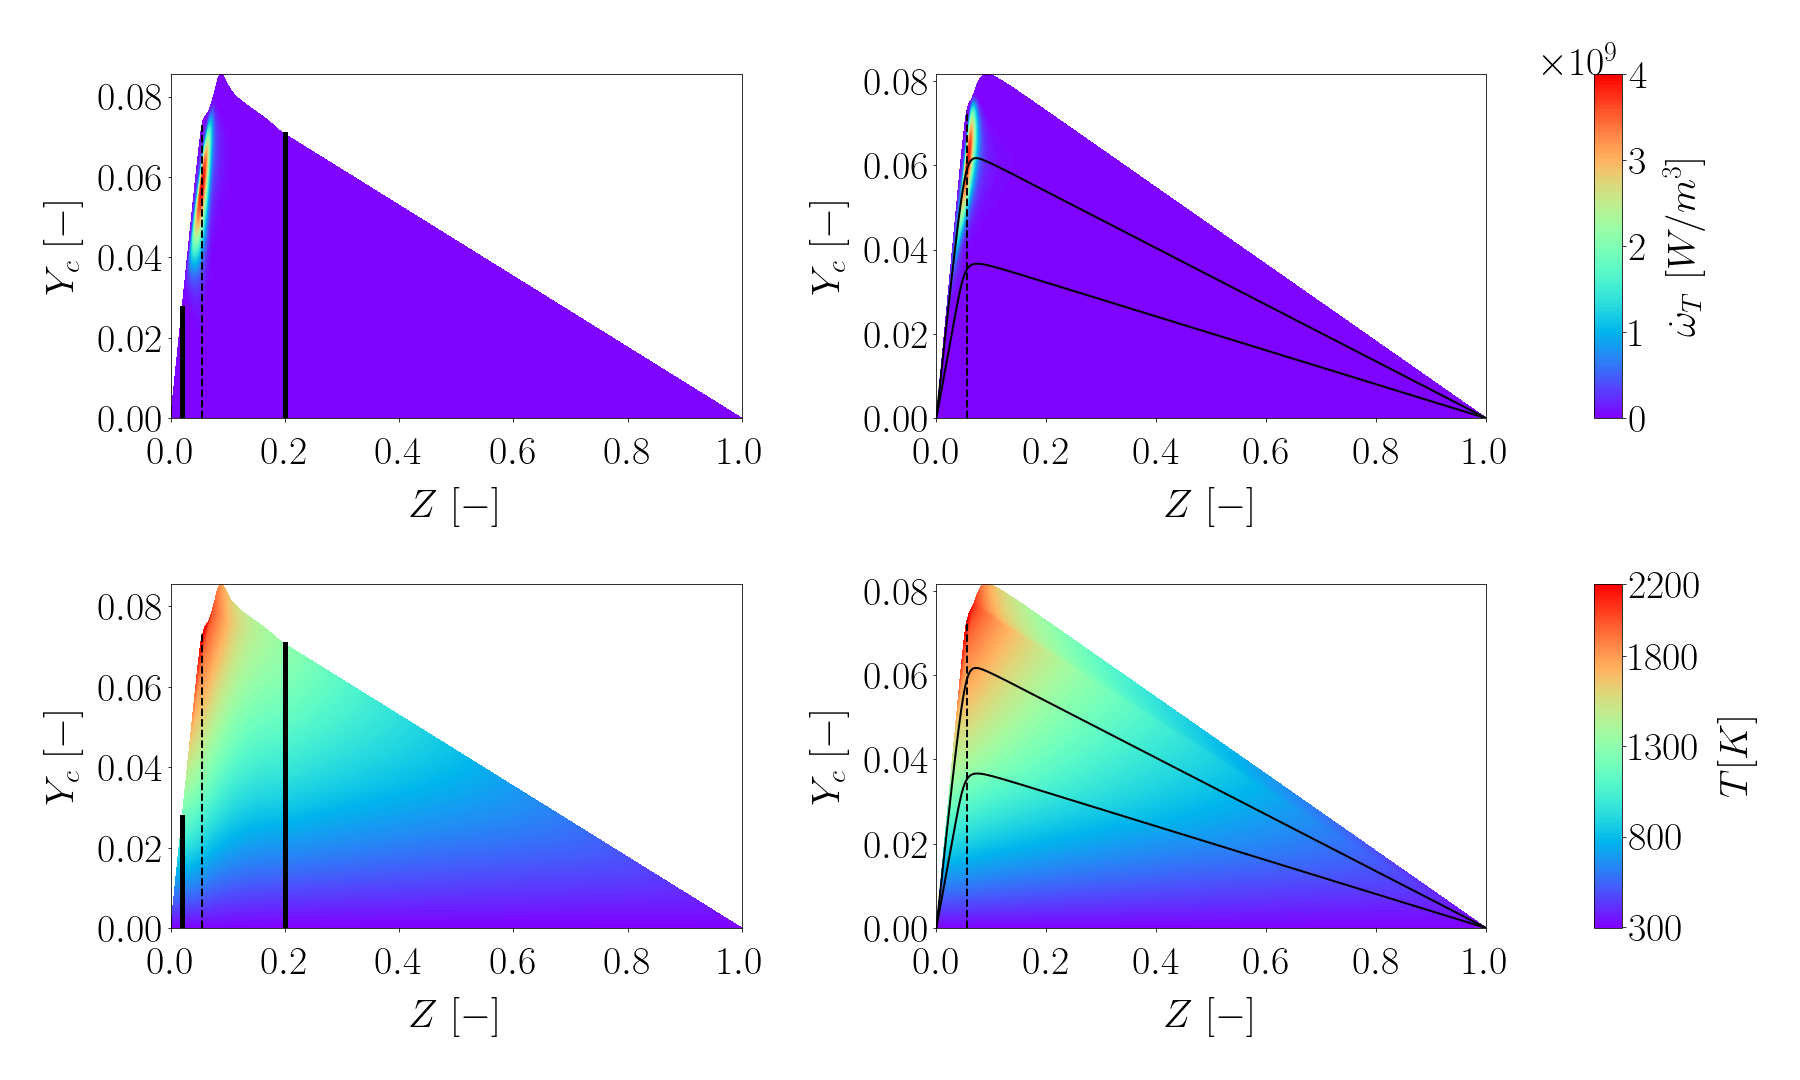
\includegraphics[scale=0.25]{./figures/flamelets_all}
% \vspace{-0.4in}
%	\caption{Flamelet manifolds representing heat release rate (\textsl{top}) and temperature (\textsl{bottom}) in $Y_c - Z$ space obtained for $CH_4$ fuel. Premixed (\textsl{left}) and diffusion (\textsl{right}) manifolds are represented. The vertical black solid lines highlight the lower and upper premixed flammability limits, while the dashed one denotes stoichiometry. The solid black flamelets in the diffusion flamelets enclose the unstable branch region of the S curve. }
%	\label{fig:flamelet_manifolds}
%\end{figure}

%For look-up of properties during the computations, it is more convenient to use a scaled progress variable $C$ for tabulation:

%\begin{equation}
%C = \frac{Y_c \left( Z \right)  - Y_c^0 \left( Z \right)}{Y_c^\mathrm{eq} \left( Z \right)  - Y_c^0 \left( Z \right)}    
%\end{equation}

%where the superscripts $0$ and $\mathrm{eq}$ denote fresh gases and equilibrium conditions respectively. With such transformation, $C = 0$ and $C = 1$ correspond to unreacted and fully reacted conditions. The pre-computed thermochemical tables are then stored as a function of variables $Z-C$. This methodology has been extensively used and validated in several cases \citep{govert_effect_2018,pachano_numerical_2023}.


\subsection{Premixedness index}
\label{subsec:premixedness_index}
%\clearpage

The distinction between premixed and non-premixed combustion is still an open area of research. One of the first attempts was introduced by \cite{yamashita_numerical_1996}, conventionally referred as Takeno index, which measures the misalignment between fuel and oxidizer. The definition is given by:

 \begin{equation}
\mathrm{TI} = \frac{\bm{\nabla} Y_f }{|\bm{\nabla} Y_f| } \cdot  \frac{  \bm{\nabla} Y_o}{ |\bm{\nabla} Y_o|} = \bm{n}_f \cdot \bm{n}_o,
\end{equation}

where $f$ and $o$ denote fuel and oxidizer, respectively.  This definition is based on the unitary vectors of fuel gradient $\bm{n}_\mathrm{f} =   \bm{\nabla} Y_\mathrm{f} / |\bm{\nabla} Y_\mathrm{f}|$  and oxidizer gradient $\bm{n}_\mathrm{o} =   \bm{\nabla} Y_\mathrm{o} / |\bm{\nabla} Y_\mathrm{o}|$, thus $\mathrm{TI}$ reflects their misalignment. When both vectors are aligned, its value is $1$ and it denotes premixed conditions. When they are misaligned, it yields $-1$ and non-premixed conditions are identified. This definition was normalized by \cite{domingo_partially_2002} to define a new index $\xi_\mathrm{TI}=[0,1]$ that is easier to interpret, where $0$ corresponds to diffusion and $1$ corresponds to premixed conditions:

\begin{equation}
    \label{eq:zeta_TI}
    \xi_\mathrm{TI} = \frac{1}{2} \left( \mathrm{TI} + 1 \right) = \frac{1}{2} \left( \frac{\bm{\nabla} Y_\mathrm{f} }{|\bm{\nabla} Y_\mathrm{f}| } \cdot  \frac{  \bm{\nabla} Y_\mathrm{o}}{ |\bm{\nabla} Y_\mathrm{o}|}  + 1 \right)
 \end{equation}

The Takeno index has been widely used as a postprocessing tool for evaluating premixed and diffusion regions in a variety of flames~\citep{hannebique_large_2013,laera_stabilization_2021}, though it has
certain limitations, as pointed 
out by~\cite{zirwes_identification_2021}. Besides, it provides values of $0$ or $1$, with a step transition among them. This hinders its application as a flame index to base multiregime methods, where a smooth transition among regimes is required to avoid numerical instabilities \citep{kleinheinz_computational_2017}. Furthermore, it fails at identifying the burning regime in the vicinity of the stoichiometric surface in purely non-premixed flames, where combustion is diffusion-controlled but the index predicts premixedness. \cite{fiorina_approximating_2005} addressed this problem by using the ratio between the local oxidizer mass fraction gradient in the diffusion flame and the gradient of unstrained premixed flames, $D_O$, as an additional parameter to flip the index when it is greater than $1$, which occurs in the regions where Takeno fails. Other markers not based on gradients alignment have been developed for regime identification, such as the index based on drift terms of \cite{wu_compliance_2016}, which calculates an error estimator between manifolds that is species specific, and the Gradient-Free Regime Identification (GFRI) approach by \cite{butz_local_2019}, which relies on experimental data for its calculation. However, these markers differ when predicting combustion regimes in partially premixed flames \citep{zirwes_identification_2021}, and no consensus in the literature on which one should be used compared to the others has yet been reached.



%The Takeno index has been widely used as a postprocessing tool for evaluating premixed and diffusion regions in \dmm{flames~\citep{}. Despite itswidespread use, it has certain limitations, as pointed out by~\cite{zirwes_identification_2021}}, so other methods have also been derived to discriminate between premixed and non-premixed combustion, such as Gradient-Free Regime Identification (GFRI)~\citep{butz_local_2019} or the Chemical Mode Analysis~\citep{}. 


%Nevertheless, it mostly yields values of $0$ or $1$, with a step transition among both. This hinders its application as an application index to base multiregime methods, where a smooth transition among regimes is required to avoid numerical instabilities \citep{kleinheinz_computational_2017}. Furthermore, it fails at identifying the burning regime in the vicinity of the stoichiometric surface in purely non-premixed flames, where combustion is diffusion-controlled but the index predicts premixedness. \cite{fiorina_approximating_2005} addressed this problem by using the ratio between the local oxidizer mass fraction gradient in the diffusion flame and the gradient of unstrained premixed flames, $D_O$, as an additional parameter to flip the index when it is greater than $1$, which occurs in the regions where Takeno fails. Other markers not based on gradients alignment have been developed for regime identification, such as the index based on drift terms of \cite{wu_compliance_2016}, which calculates an error estimator between manifolds that is species specific, and the Gradient-Free Regime Identification (GFRI) approach by \cite{butz_local_2019}, which relies on experimental data for its calculation. However, these markers differ when predicting combustion regimes in partially premixed flames \citep{zirwes_identification_2021}, and no consensus in the literature on which one should be used compared to the others has yet been reached.

The use of a flame index for tabulated chemistry that could combine different chemical manifolds offers great potential to deal with the limitations of conventional databases based on one-dimensional manifolds, while retaining the simplicity of the generation of flamelet tables~\citep{knudsen_capabilities_2012,kleinheinz_computational_2017,butz_local_2019}. In our previous work~\citep{illana_extended_2021}, we proposed a new flame index definition for multiregime phenomena based on the control variables of the chemical manifold, so the index can be directly applied to flamelet calculations. The proposed premixedness index is given by:


%In this work, to circumvent the aforementioned issues and also use the flamelet variables $Z-Y_c$ to allow its application in simulations with flamelet approaches, the following definition by \cite{illana_extended_2021} is used:

\begin{equation}
    \label{eq:zeta_PF_illana}
\xi_\mathrm{PF} = k \left( 1 - \frac{\nabla Z}{|\nabla Z|^\mathrm{diff}} \cdot \frac{\nabla Y_c}{|\nabla Y_c|} \right),
\end{equation}

where the numerator $|\nabla Z|^\mathrm{diff}$, which depends on $Z$ and $Y_c$, represents the magnitude of the mixture fraction gradient of a one-dimensional strained counterflow diffusion flame. The use of this variable ensures that the dot product does not produce abrupt jumps from one limit to the other, ensuring a smooth transition between regimes as required to avoid numerical instabilities \citep{kleinheinz_computational_2017}. The parameter $k$, which depends on $Z$, is a correction factor to account for the influence of the lean and rich flammability limits of one-dimensional premixed flames. It takes a value of $1$ within the premixedness limits, a value of $0$ far from the limits, and there is an exponential but smooth transition between $1$ and $0$ close to the flammability limits. In this way, only diffusion characteristics are obtained away from the flammability limits determined by the premixed flamelets, where solutions for premixed combustion do not exist. This flame index is used to weight locally the contributions of the flamelet libraries:

\begin{equation}
    \dot{\omega}_{Y_c}^\mathrm{TC} = \xi_\mathrm{PF} \cdot\dot{\omega}_{Y_c}^\mathrm{PTC}  \left( Z, Y_c \right) + \left( 1 - \xi_\mathrm{PF} \right) \cdot \dot{\omega}_{Y_c}^\mathrm{DTC} \left( Z, Y_c \right),
\end{equation}


where PTC and DTC refer to tabulated premixed and diffusion flamelets respectively, while TC denotes the tabulated quantity resulted from the application of the index. In this work, the use of the Takeno index is retained to facilitate the comparisons with the premixedness index and cross-correlate the identification of multiregime phenomena.
%with blended properties. 

%\subsubsection*{Recovery of pure diffusion limit}

\subsubsection*{Capturing the asymptotic diffusion limit of combustion}

The use of a flame index for blending chemical manifolds must satisfy certain requirements. The index should
recover the two asymptotic limits of combustion: premixed ($\xi_\mathrm{PF} = 1$) and non-premixed ($\xi_\mathrm{PF} = 0$), 
while it must be smooth across the transitions to avoid numerical instabilities. In the first study~\citep{illana_extended_2021}, it was shown the flame index was able to recover not only the premixed limit, simply by its definition ($\nabla Z = 0$), but also partially premixed combustion with different mixing lengths across a variety of conditions. However, the computational cases presented there did not approach the asymptotic limit of non-premixed combustion. This is a more challenging requirement for a flame index as it requires the use of two independent and orthogonal coordinates to describe the chemical manifold~\citep{mueller_physically-derived_2020,scholtissek_derivation_2020}. 

This aspect can be distinguished in Fig.~\ref{fig:flame_1D_flame_index} considering a 1D counterflow diffusion flame in physical space.
$\xi_\mathrm{PF}$ is $0$ along most of the domain except at high values of the progress variable $C$. The reason for this prediction can be seen in the right graph of Figure \ref{fig:flame_1D_flame_index}, where the gradients $\nabla Z$, $\nabla C$ and the dot product $\nabla Z \cdot \nabla C$ are plotted. In the region of the highest progress variable, the gradients $\nabla Z$ and $\nabla C$ are counter-aligned, hence the dot product is negative resulting in $\xi_\mathrm{PF}$ being larger than $1$. Furthermore, the transition from $\xi_\mathrm{PF} = 0$ to higher values is steep since it enters the flammable region, where $k = 1$, therefore creating discontinuities when applied in reactive computations. 
The Takeno index also encounters these limitations, as shown in Fig.~\ref{fig:flame_1D_flame_index}.

%Since the flame index must accurately identify the premixed and non-premixed limits, $\xi_\mathrm{PF} = 0$ is expected in purely premixed cases and $\xi_\mathrm{PF} = 0$ in purely diffusion flames. The first case always holds, for example, in a 1D premixed flame where $\nabla Z = 0$. 

%However, $\xi_\mathrm{PF} = 0$ is not always predicted in non-premixed flames. 
%Fig.~\ref{fig:flame_1D_flame_index} shows a 1D counterflow diffusion flame in physical space. When Eq. (\ref{eq:zeta_PF_illana}) is applied, 


\begin{figure}[h!]
	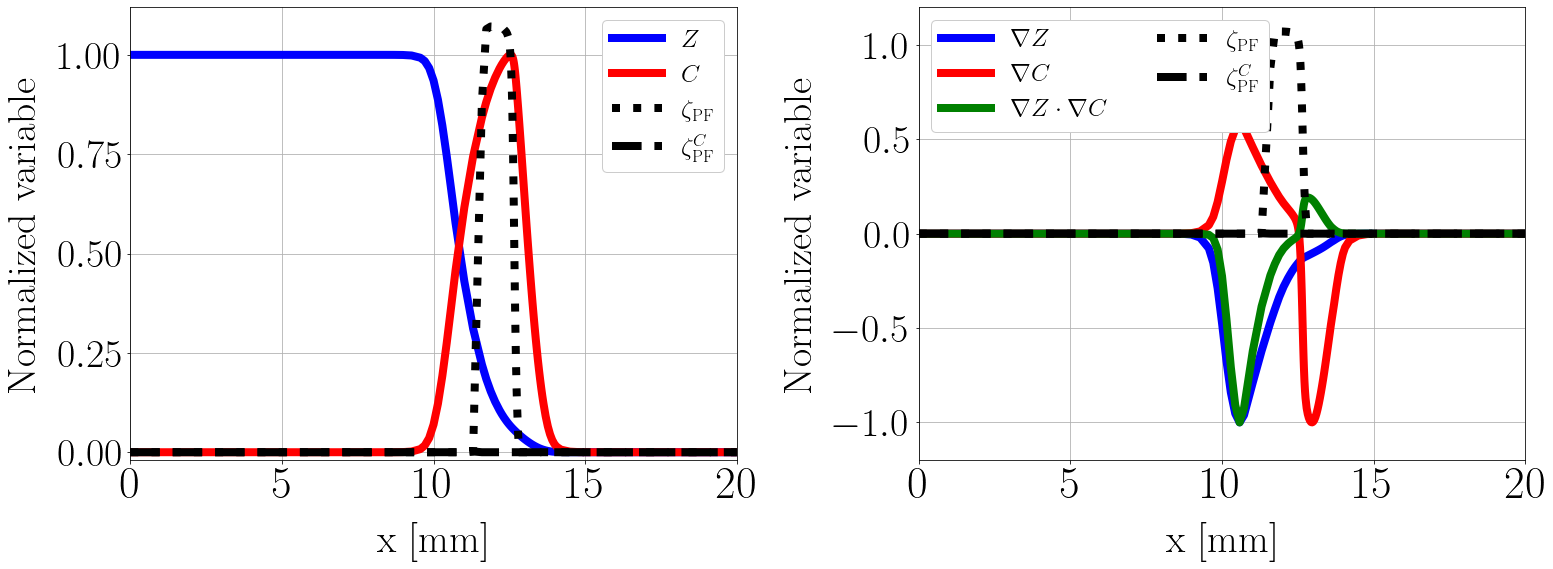
\includegraphics[scale=0.25]{./figures/flame_1D_flame_index}
    %\vspace{-0.5in}
	\caption{Flame index predictions in a CH4/air 1D counterflow diffusion flame. The left plot shows $Z$ and $C$ in the physical space. The right plot shows their gradients and the dot product employed in the calculation.} 
	\label{fig:flame_1D_flame_index}
\end{figure}

Quadrants sketch in Fig.~\ref{fig:quadrants_sketch}.

\begin{figure}[h!]
\centering
	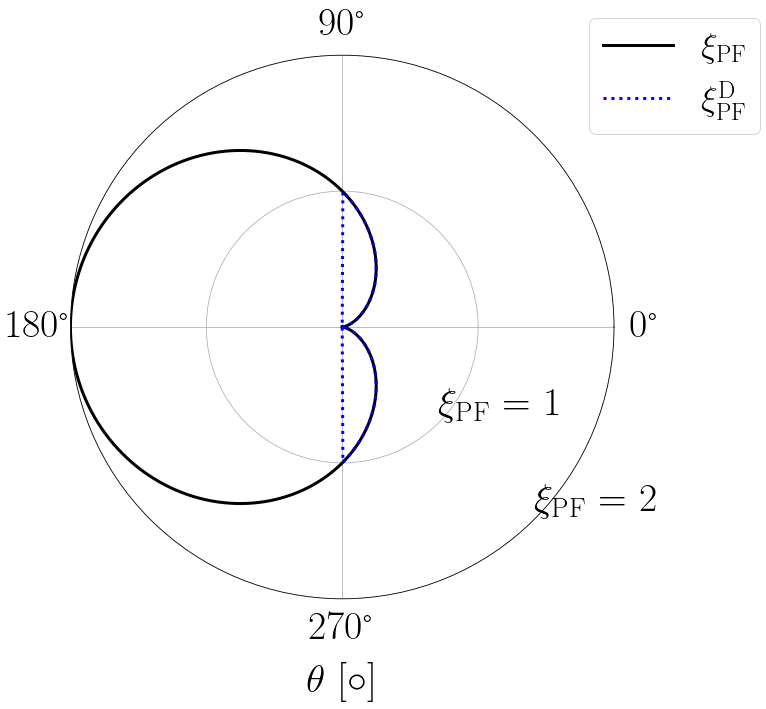
\includegraphics[scale=0.2]{./figures/quadrants_polar_sketch}
    %\vspace{-0.5in}
	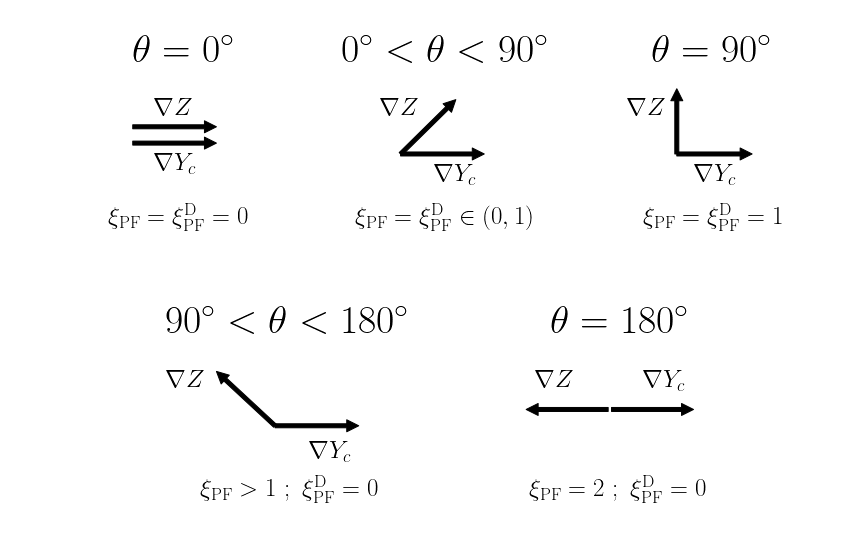
\includegraphics[scale=0.25]{./figures/quadrants_arrows_gradients}
	\caption{Quadrants} 
	\label{fig:quadrants_sketch}
\end{figure}

\dmm{\textsl{WE SHOULD REVISE THE TEXT ABOVE BASED ON THE NEW CORRECTION OF THE MODEL. }}


%To mitigate this shortcoming, a threshold is applied for limiting $\xi_\mathrm{PF}$ to $0$ in regions where $\xi_\mathrm{PF} > 1$. The application of the flame index prediction when the threshold is applied is denoted by variable $\xi_\mathrm{PF}^C$ in Figure \ref{fig:flame_1D_flame_index}. As observed, with this modification the flame index predicts $0$ all over the flame, therefore recovering the diffusion limit. Hereafter, this modification will be applied to all cases and will be solely referred as $\xi_\mathrm{PF}$. A comparison of flamelet computations for two cases with and without applying this correction is reported in \ref{sec:app_index_with_without_threshold}.

%\clearpage

\section{Computational setup}
\label{sec:computational_setup}

%\clearpage

The planar coflow configuration considered for this study is shown in Figure \ref{fig:simu_config}. This configuration is similar to other coflow geometries studied in previous works using tabulated chemistry methods \citep{consul_analysis_2008}. The flow condition is determined by a central injector (primary) with an outer injector or coflow (secondary inlet). This configuration can recreate a wide range of conditions from premixed or diffusion flames to partially premixed flames with different level of multiregime phenomena by simply adjusting the flow rates and equivalence ratios of the different inlets. {This case also allows to evaluate the ability of the proposed flame index to approximate the diffusion limit and quantify the disagreements with respect to the flamelet methods with single manifold representation.

\dmm{\emph{@anurag: shall we mention something about the scalar dissipation rates here?}}


Due to burner symmetry, only half of the domain is solved and a symmetric boundary condition is specified at the left side, thereby reducing the computational cost. All the burner walls are set as no-slip and adiabatic, hence the flames are confined. The computational domain is discretized with a structured mesh composed of square elements with regular size $\Delta x = 20~\mu$m. 


\begin{table}[h!]
\centering
\caption{Injection equivalence ratios and velocities in simulated cases.}
\begin{tabular}{ccccc}
\hline
Case & $\Phi_p$ {[}-{]} & $\Phi_m$ {[}-{]} & $u_p$ {[}m/s{]} & $u_m$ {[}m/s{]} \\ \hline
0             & $\infty$     &  0               & 0.1                      & 0.5                      \\ 
A             & $\infty$     & 0.3                & 0.1                      & 0.5                      \\ 
B             &  $\infty$    & 0.8                 & 0.1                      & 1.3                      \\ 
C             &  2           & 0.3              & 0.1                      & 0.5                      \\ 
D             &  2           & 0.8              & 0.1                      & 1.3                      \\ \hline
\end{tabular}
\label{tab:BCs_simulations}
\end{table}



The different computational cases with their associated boundary conditions in terms of equivalence ratio $\Phi$ and inlet velocities are shown in Table \ref{tab:BCs_simulations}. A total of five different flow conditions have been selected that feature different types of multiregme phenomena. Cases featuring a  diffusion flame on the central injector interacting with a non-flamable mixture for the coflow are considered for cases A and B, while the interactions between rich and lean partially premixed flames are considered for cases C and D. Additionally, a pure diffusion coflow flame has also been considered as reference (Case 0), where pure air is injected through the secondary inlet and pure fuel through the primary injector. As the focus of the study is to describe multiregime phenomena, a simple fuel (methane $CH_4$) with well-established chemistry is considered.
%, The selected fuel for the study is methane due to the well-kno is used as fuel in all cases. 





%The geometry of the computed burner is displayed in Figure \ref{fig:simu_config}. Two inlets are present, a central injector (pilot inlet) and an outer one (main inlet), through which air and fuel can be introduced in the domain at different equivalence ratios, therefore recreating partially premixed conditions. Due to burner symmetry, only half of the domain is solved and a symmetric boundary condition is specified at the left side, thereby reducing computational costs. The outer and between-inlets walls are set as no-slip adiabatic, hence the flames are confined. For spatial discretization of the domain, a structured mesh composed of square elements with size $\Delta x = 50~\mu$m is used. 

%The boundary conditions in terms of inlet equivalence ratios $\Phi$ and velocities for the simulated cases are shown in Table \ref{tab:BCs_simulations}. These are identical in all DC and TC computations. Methane $CH_4$ is used as fuel in all cases. A total of 5 simulations have been performed, where the equivalence ratios are varied to recreate partially-premixed conditions which can be more diffusion-like (cases A and B) or premixed-like (cases C and D). Additionally, a pure diffusion coflow flame has also been computed (case 0), where pure air is injected through the main inlet and pure methane through the coflow one. 



\begin{figure}[h!]
	\centering
	%
\includegraphics[scale=0.8]{./figures/simu_config}
 \includeinkscape[scale=0.75]{./figures/simu_config}
	\caption{Geometrical setup. Dimensions are in mm (not to scale). Each color denotes a different boundary condition type.}	
	\label{fig:simu_config}
\end{figure}

\section{Results and discussion}
\label{sec:results_discussions}
%\clearpage

\dmm{\emph{WE SHOULD EXPLAIN HERE THE WHOLE SECTION AND WHAT WILL BE PRESENTED}}

%\subsection{Direct chemistry simulations}

\subsection{Analysis of the multiregime penomena for the different flow conditions}

The flow fields for mixture fraction and temperature at steady state conditions for the cases in Table \ref{tab:BCs_simulations}  are shown in the top and middle plots of Fig.~\ref{fig:FR_maps_T_TI}. The plots are presented with normalized dimensions to facilitate the comparison using the secondary inlet diameter $D = 3~\mathrm{mm}$ for scaling, see Fig.~\ref{fig:simu_config}. The mixture fraction fields show the different stratification levels obtained in each case. The location of the stoichiometric condition $Z_\mathrm{st} = 0.055$ is denoted by the red contour. In cases 0, A and B the stoichiometric line extends downstream from the injector lip separating the lean region at the right side from the rich one at the left part of the domain. These cases present high stratification, since the mixture fraction runs from $1$ in the central injector to lower values (0 in case 0 and $0.027$, corresponding to $\phi = 0.8$, in cases B and C) in the coflow. Cases C and D present a stoichiometric line that extends from the injector lip towards the centerline. This line encloses rich mixtures close to the central injector, while leaner ones are located outside. Temperature fields are shown at the middle row, where the yellow lines denote the contours $ \dot{\omega}_T /\max \left( \dot{\omega}_T \right)  = 0.1 ~ \%$ to highlight the regions of high heat release. The stoichiometric line is comprised within the reactive region in all cases. For the cases with a coflow mixture within the flammability limits (cases B and D), a premixed Bunsen flame is stabilized at the exit of the outer injector. Since $\phi = 0.8$ in these flames, the remaining fuel in the products burns with the fuel coming from the central injector, leading to an extension of the reactive region. In cases where the central injector delivers pure fuel (cases 0, A and B), reactions extend downstream in a narrow region where pure fuel and oxidizer reach through opposite sides, hence corresponding to a diffusion branch. The other cases (C and D) feature a reaction area more concentrated around the injectors. The highest temperatures are located within the reaction regions, around the stoichiometric line. Outside those, temperature differences due to heating from the products are found in cases 0, A and C, while cases B and D present high temperatures outside the reactions corresponding to the burnt gases from the Bunsen flame.

The bottom row of Fig.~\ref{fig:FR_maps_T_TI} shows the scaled Takeno Index $\xi_\mathrm{TI}$ calculated with Eq.~(\ref{eq:zeta_TI}), which is used here to discrimite between 
premixed- and diffusion-dominated combustion. In cases 0 and A, $\xi_\mathrm{TI}$ predicts diffusion in the inner part of the reactive layer and premixed combustion in the outer part. This index transition is the aforementioned misprediction due to the  gradients of fuel and oxidizer pointing in the same direction, causing the Takeno index to predict premixedness instead of diffusion as such gradient alignment occurs on the lean side \citep{fiorina_approximating_2005}. When the amount of fuel increases within the flammability limits (case B), the purely premixed nature of the Bunsen flame is correctly identified and diffusion is detected elsewhere. If primary injection changes from pure fuel to a premixed mixture (cases C and D), the reactivity of the mixture increases around the central region close to the injector, premixed and diffusion combustion also coexist with a predominance of the former. The multiregime nature of these flames,  where some of them are dominated by diffusion (cases 0, A, C) and others by flame propagation (cases B and D) 
is thus manifested in the $\xi_\mathrm{TI}$ distribution.



%Resulting fields from the DC computations for the cases of Table \ref{tab:BCs_simulations} are shown in Figure \ref{fig:FR_maps_T_TI}. Spatial coordinates are shown in dimensionless form by dividing with respect to the diameter of the main inlet $D = 3~\mathrm{mm}$. Displayed fields are the mixture fraction $Z$, the temperature and the scaled Takeno index $\xi_\mathrm{TI}$. 
    
%The $Z$ field shows the different stratification levels in each case. The location of stoichiometric conditions $Z_\mathrm{st} = 0.055$ is denoted by the red contour. Temperature fields are shown at the middle row, where the yellow lines denote the contours $ \frac{\dot{\omega}_T }{\max \left( \dot{\omega}_T \right) } = 0.1 ~ \%$ to highlight the regions of high heat release. The stoichiometric line is comprised within the reactive region in all cases. For simulations with a main mixture within the flammability limits (cases B and D), this mixture ignites and forms a Bunsen flame stabilizing at the exit of the main inlet tube, which is a characteristic premixed flame. The rest of the cases, with a main mixture below the lower flammability limit, do not show this feature. The bottom row shows the scaled Takeno Index $\xi_\mathrm{TI}$ given by the following definition:



%where $Y_f$ and $Y_o$ represent the mass fractions of fuel and oxidizer, respectively. With this definition, which measures the orientations of fuel and oxidizer gradients, premixed combustion is identified as $\xi_\mathrm{TI} = 1$ while diffusion regions correspond to $\xi_\mathrm{TI} = 0$. Case 0, where no fuel is injected through the main injector, shows a classical diffusion coflow flame where high heat release and the highest temperatures are located in a narrow band where both streams mix. The index $\xi_\mathrm{TI}$ predicts that diffusion in the inner part of the reactive layer and premixedness in the outer part. The reason for detecting this region as premixed is that gradients of fuel and oxidizer are pointing in the same direction, which is a shortcoming of the Takeno index when applied to diffusion flames since such alignment occurs in their lean side \citep{fiorina_approximating_2005}. When methane is added in the main injector below the flammability limits (case A), the reactive region gets wider and higher temperatures are found downstream. $\xi_\mathrm{TI}$ predicts again diffusion in the fuel side and premixedness in the oxidizer side. If the percentage of $CH_4$ is increased within the flammability limits (case B), higher temperatures are present in the domain, specially closer to the lateral walls, as a consequence of burnt gases coming from the premixed Bunsen flame. The index $\xi_\mathrm{TI}$ shows that both premixed and diffusion modes coexist in both regions, and is able to detect the fully premixed nature of the Bunsen flame. If the pilot injection is now changed from pure $CH_4$ to a premixed mixture (cases C and D), reactivity increases around the central region close to the pilot injector, and hence the highest temperatures are also shifted towards the middle of the domain. The effect of dilution in the main injector has a similar behavior as in the previous cases: premixed and diffusion regimes coexist in the reactive layer when the main mixture is below the flammability limits (case C), and a premixed Bunsen flame is formed if the equivalence ratio is increase to 0.8 (case D). The multiregime nature of these flames, where some of them are dominated by diffusion (cases 0, A, C) and other are more premixed-like (cases B and D), is therefore manifested in the $\xi_\mathrm{TI}$ distribution.





\begin{figure}[h!]
    %\hspace{-0.5in}
    \centering
	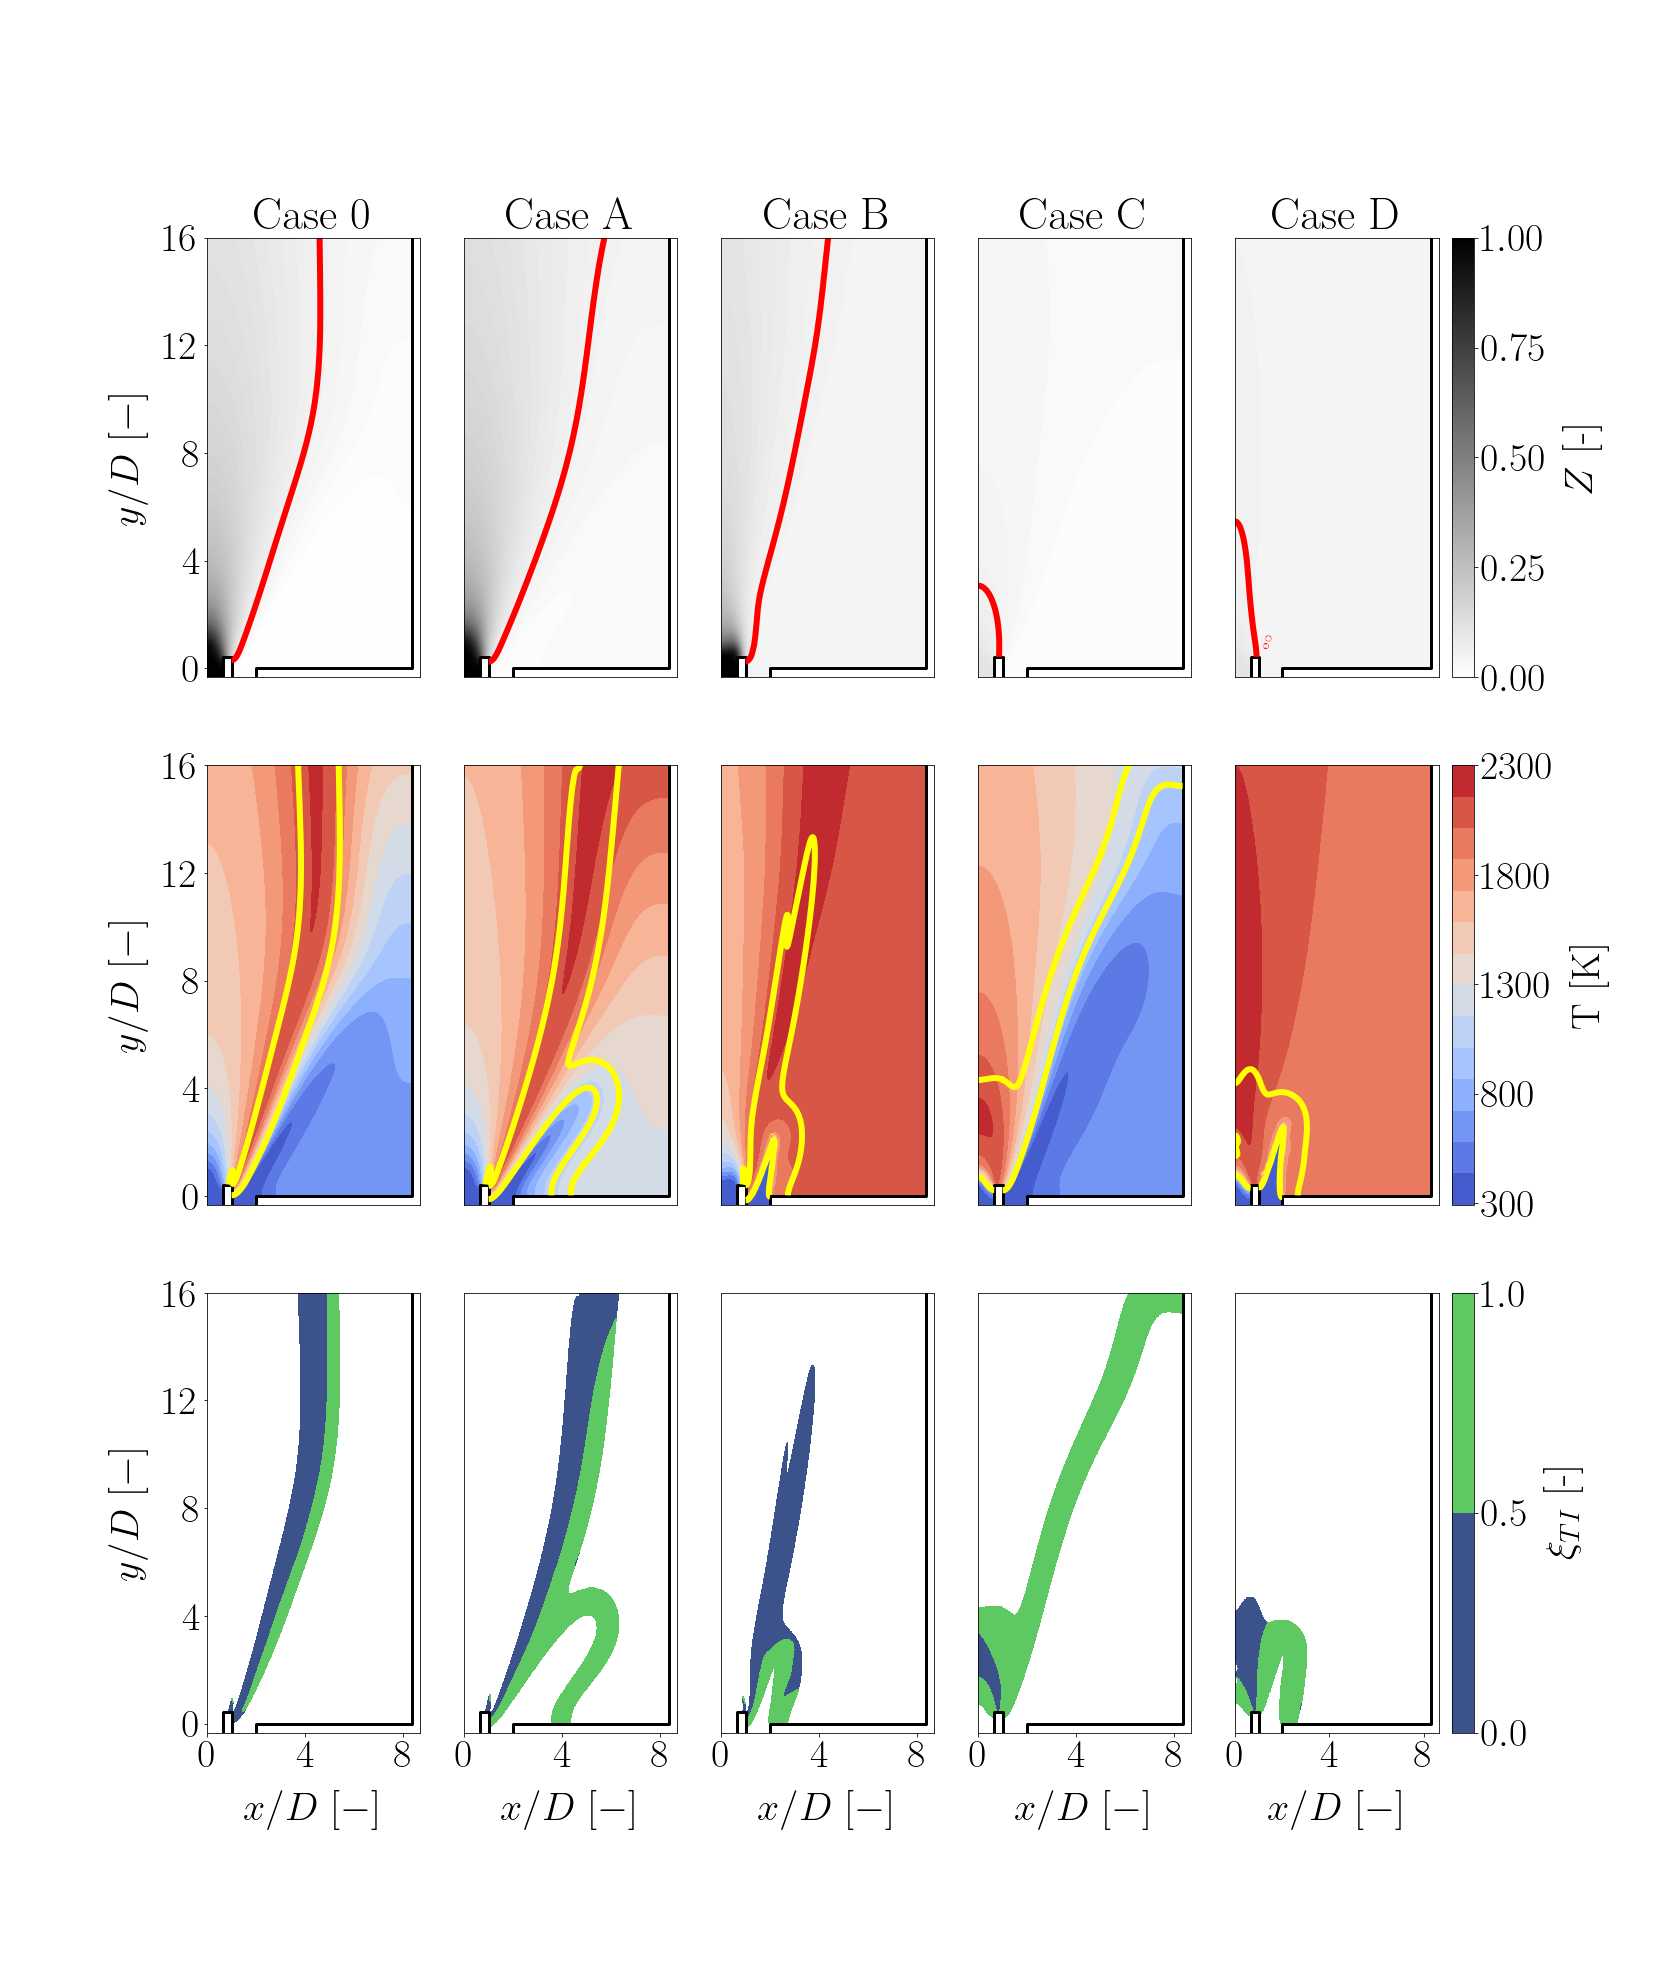
\includegraphics[scale=0.25]{./figures/FR_maps_Z_T_zetaTI}
    \vspace{-0.5in}
	\caption{Results of DC computations. The red solid line at the top row corresponds to the contour $Z = Z_\mathrm{st}$. The yellow lines at the middle row correspond to the contour of heat release $ \frac{\dot{\omega}_T }{\max \left( \dot{\omega}_T \right) } = 0.001$, while the index $\xi_\mathrm{TI}$ is shown at the bottom row clipped to high reactive regions where $ \dot{\omega}_T >  0.001 \max \left( \dot{\omega}_T \right)$.}
	\label{fig:FR_maps_T_TI}
\end{figure}

\clearpage

\subsection{\textsl{A priori} analysis of the proposed premixedness index}

In this sub-section, the proposed premixed index for tabulated 
chemistry (Eq. \ref{eq:zeta_PF_illana}) is evaluated \textsl{a priori} using the flow fields generated from the detailed chemistry solutions. For its application, the progress variable and mixture fraction are defined directly from the species mass fractions, and the gradients of $Z$ and $Y_c$ are computed from the resolved fields. The index also needs the magnitude of $|\nabla Z|^\mathrm{diff}$, which is interpolated  from the diffusion flamelet manifold at each spatial location  from its corresponding $(Z,Y_c)$ coordinates, as this quantity is also part of the manifold  $|\nabla Z|^\mathrm{diff}=f(Z,Y_c)$. The premixedness index, estimated a priori from the DC results, is denoted as $\xi_\mathrm{PF}^\mathrm{DC}$.

Additionally, an index $\xi_\mathrm{id}$ is introduced 
to ideally capture the characteristics of the DC calculations. Using the heat release rate field from the DC solution, represented as $\dot{\omega}_{T}^\mathrm{DC}$, this index interpolates the properties from the premixed and diffusion flamelet manifolds, 
$\mathrm{PTC}$ and $\mathrm{DTC}$ respectively, as follows:

%This premixedness index estimated a-priori from the 
%DC results is labelled as $\xi_\mathrm{PF}^\mathrm{DC}$. 

%Additionally, an index $\xi_\mathrm{id}$ is defined which would ideally retrieve the characteristics of the DC computation. Using the heat release field from DC, denoted as  $\dot{\omega}_{T}^\mathrm{DC}$, this index would interpolate the properties from the premixed and diffusion flamelet manifolds, $\mathrm{PTC}$ and $\mathrm{DTC}$ respectively, such that:

\begin{equation}
\label{eq:omega_T_zeta_id_definition}
    \dot{\omega}_{T}^\mathrm{DC} \left( Z, Y_c \right) = \xi_\mathrm{id} \cdot  \dot{\omega}_{T}^\mathrm{PTC} \left( Z, Y_c \right) + \left( 1 -  \xi_\mathrm{id} \right) \cdot  \dot{\omega}_{T}^\mathrm{DTC} \left( Z, Y_c \right).
\end{equation}

From this relation, the ideal index can be obtained as:

\begin{equation}
\label{eq:zeta_id}
    \xi_\mathrm{id} = \frac{\dot{\omega}_{T}^\mathrm{DC} - \dot{\omega}_{T}^\mathrm{DTC}}{\dot{\omega}_{T}^\mathrm{PTC} - \dot{\omega}_{T}^\mathrm{DTC}}.
\end{equation}


The distribution of the premixed $\xi_\mathrm{PF}^\mathrm{DC}$ and 
Takeno $\xi_\mathrm{TI}$ indexes restricted to the high reactive 
regions where $\dot{\omega}_T > 0.1~\% $ of the maximum value from $\dot{\omega}_{T}^\mathrm{DC}$ are shown 
in Fig.~\ref{fig:FR_maps_a_priori_zetas} for cases 0, A and B. These have been chosen because they include all multiregime features of interest, and cases C and D are similar to A and B respectively. The results indicate that both indices accurately predict the location of the reacting layers, although they differ in how they handle the transition from diffusion-dominated flames (Case 0) to partially and fully premixed flames (Cases A and B). The ideal index, $\xi_\mathrm{id}$, suggests that the flame can be characterized by a combination of the two manifolds (premixed and diffusion), but this approach introduces strong oscillations and discrete variations in the premixed index used for interpolating between solutions. Similarly, the Takeno index, $\xi_\mathrm{TI}$, also displays sharp gradients and discontinuities between solutions, reflecting abrupt transitions between combustion modes. In contrast, the premixed index based on flamelet variables, $\xi_\mathrm{PF}^\mathrm{DC}$, provides smooth transitions between thermal states, which could help avoiding spurious oscillations at the flame front. This behavior is particularly beneficial for maintaining numerical stability and physical continuity in simulations. In the limit of non-premixed combustion, as seen in Case 0 (pure diffusion flame), the proposed index $\xi_\mathrm{PF}^\mathrm{DC}$ accurately predicts the formation of a pure diffusion flame, aligning well with the ideal index $\xi_\mathrm{id}$. However, the Takeno index, $\xi_\mathrm{TI}$, is unable to recover this limit, consistent with findings reported in previous studies \citep{fiorina_approximating_2005,zirwes_identification_2021}. In Case A, where a lean premixed mixture is injected from the outer layer and interacts with the diffusion flame originating from the central injection, the index $\xi_\mathrm{PF}^\mathrm{DC}$ predicts a thinner premixed front in the outer layer compared to the ideal index, while the Takeno index successfully captures this transition. For Case B, which involves two perfectly premixed flames, both $\xi_\mathrm{PF}^\mathrm{DC}$ and $\xi_\mathrm{TI}$ accurately recover the premixed combustion limit, as indicated by the ideal index. Overall, the index $\xi_\mathrm{PF}^\mathrm{DC}$ demonstrates a strong capability to recover both combustion limits while maintaining smooth transitions between regimes. This smooth behavior facilitates the direct application of this index to practical combustion scenarios, offering a balanced approach that minimizes spurious numerical artifacts while accurately representing physical combustion processes.

\clearpage



%The index $\xi_\mathrm{PF}^\mathrm{DC}$ exhibits a smooth, continuous 
%distribution throughout the domain, whereas both $\xi_\mathrm{TI}$ 
%and $\xi_\mathrm{id}$ display discrete variations.


%Figure \ref{fig:FR_maps_a_priori_zetas} shows the index fields clipped to high reactive regions for cases 0, A and B. The scaled Takeno index $\xi_\mathrm{TI}$ is also plotted. 

%As observed, index $\xi_\mathrm{PF}^\mathrm{DC}$ shows a continuous distribution, while  $\xi_\mathrm{TI}$ and $\xi_\mathrm{id}$ vary discretely throughout the domain. 


%In case 0, which corresponds to a pure diffusion jet, $\xi_\mathrm{PF}^\mathrm{DC}$ predicts diffusion in the displayed area. The ideal index predicts also diffusion in the outer part of the branch, which $\xi_\mathrm{TI}$ identifies as premixed. 

%For case A, $\xi_\mathrm{PF}^\mathrm{DC}$ identifies a wider predominance of diffusion than the other two definitions, and pre-mixedness is detected by all indices in the outer reactive region outside the main injector. 

%Regarding case B, premixedness is always identified around the characteristic Bunsen flame, indicating the capability of all definitions to successfully capture premixed combustion. Overall, $\xi_\mathrm{PF}^\mathrm{DC}$ can identify a great extent of regions exhibiting diffusion than the other two definitions.



\begin{figure}[h!]
    \hspace{-0.5in}
	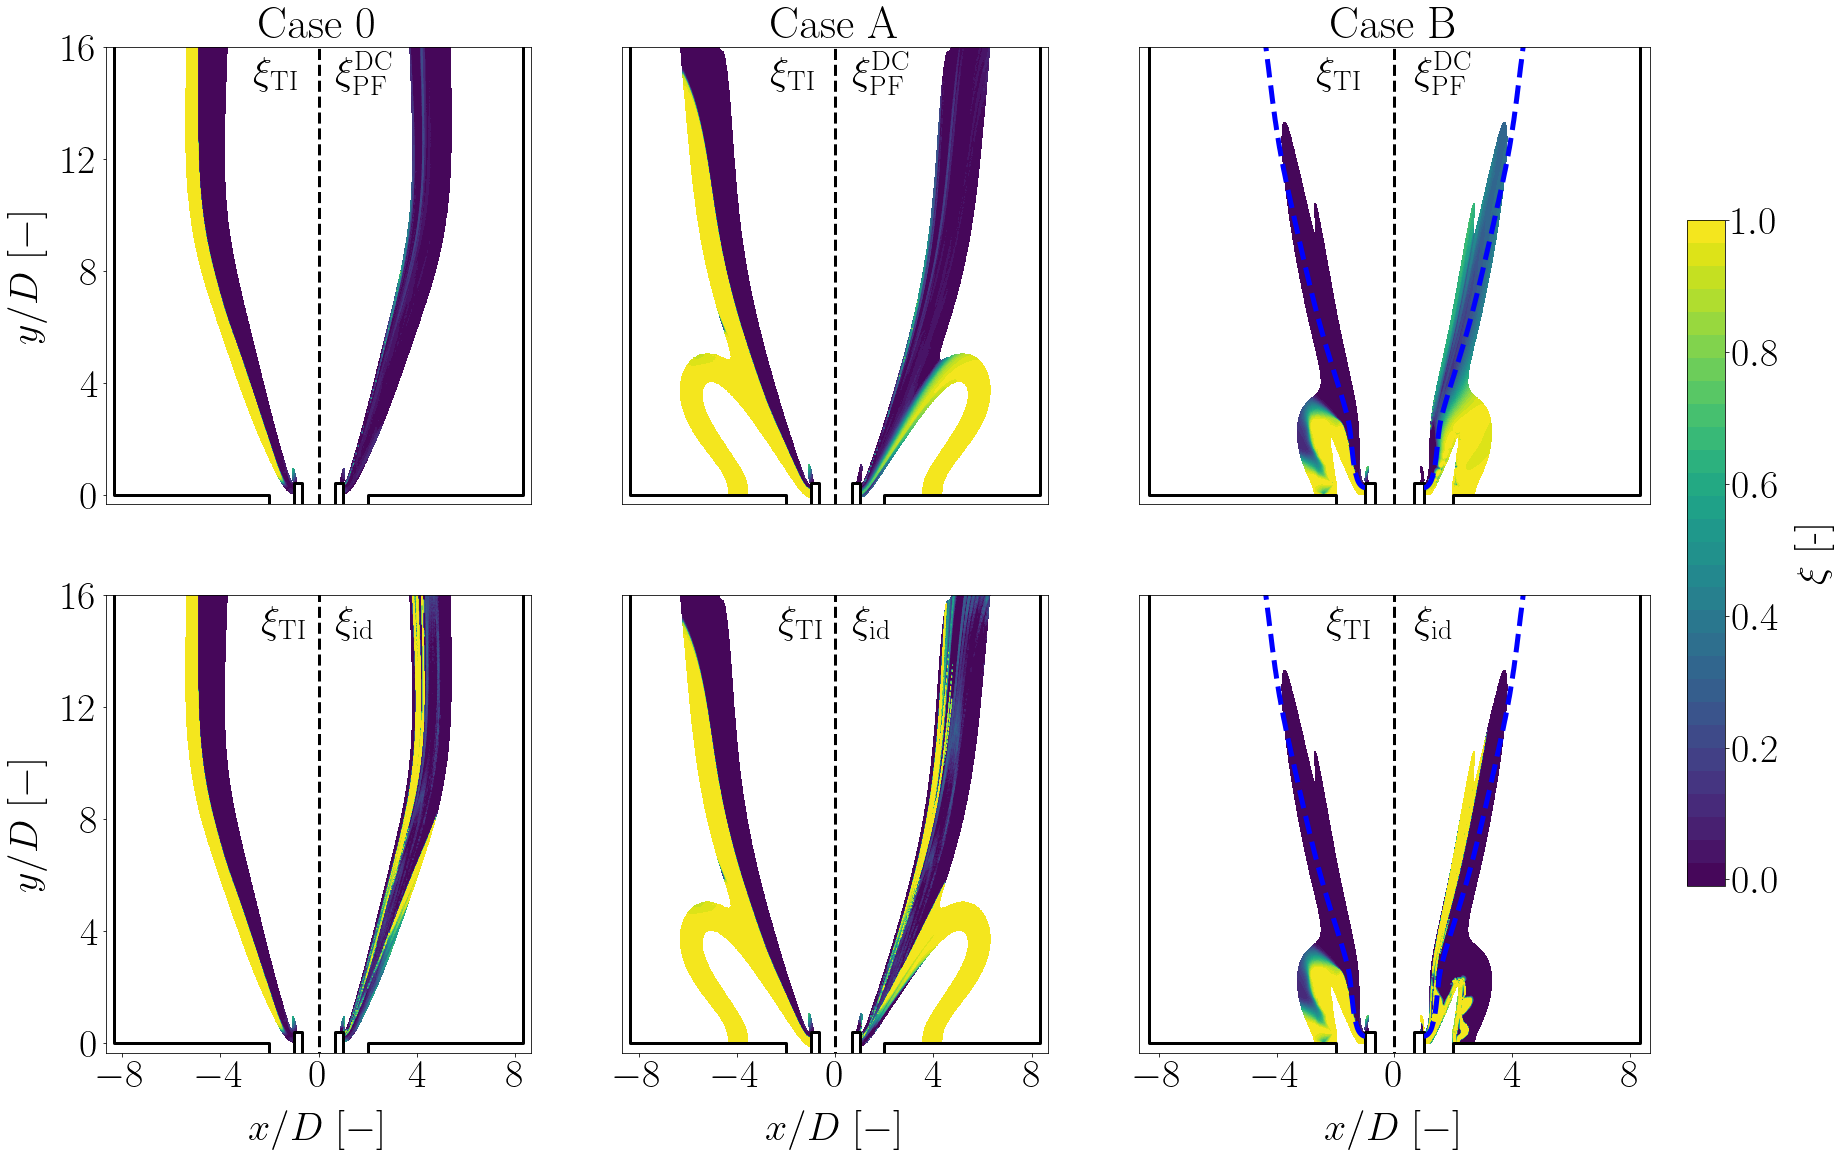
\includegraphics[scale=0.25]{./figures/FR_maps_a_priori_zetas}
    %\vspace{-0.5in}
	\caption{\textsl{A priori} analysis of flame indices fields for cases 0, A and B. The blue contour in case B corresponds to $Z = Z_\mathrm{st}$.}
	\label{fig:FR_maps_a_priori_zetas}
\end{figure}

The performance of the premixedness index $\xi_\mathrm{PF}^\mathrm{DC}$ is now assessed by reconstructing the heat release rate distribution for the  three different flames. Results for the Takeno index are also included for reference and comparison. The heat release rates for each case can be computed directly from the definition:
%As done in Eq. (\ref{eq:omega_T_zeta_id_definition}) for defining $\xi_\mathrm{id}$, similarly heat release fields can be defined by interpolating the flamelet properties with the scaled Takeno and premixedness indices:


%Performance of indices $\xi_\mathrm{TI}$ and $\xi_\mathrm{PF}^\mathrm{DC}$ can now be assessed by using them to reconstruct fields of heat release rate from the DC data. As done in Eq. (\ref{eq:omega_T_zeta_id_definition}) for defining $\xi_\mathrm{id}$, similarly heat release fields can be defined by interpolating the flamelet properties with the scaled Takeno and premixedness indices:

    \begin{equation}
    \label{eq:HRR_reconstr_PF}
    \dot{\omega}^{\xi_\mathrm{PF}^\mathrm{DC}}_{T} = \xi_\mathrm{PF}^\mathrm{DC} \cdot  \dot{\omega}_{T}^\mathrm{PTC} \left( Z, Y_c \right) + \left( 1 -  \xi_\mathrm{PF}^\mathrm{DC} \right) \cdot  \dot{\omega}_{T}^\mathrm{DTC} \left( Z, Y_c \right), 
    \end{equation}


    \begin{equation}
    \label{eq:HRR_reconstr_TI}
    \dot{\omega}^{\xi_\mathrm{TI}}_{T} = \xi_\mathrm{TI} \cdot  \dot{\omega}_{T}^\mathrm{PTC} \left( Z, Y_c \right) + \left( 1 -  \xi_\mathrm{TI} \right) \cdot  \dot{\omega}_{T}^\mathrm{DTC} \left( Z, Y_c \right).
    \end{equation}

The distribution of the heat release fields including the DC $\dot{\omega}_{T}^\mathrm{DC}$ for the three cases is shown in Fig. \ref{fig:FR_maps_a_priori_HRR}. The plot shows a good qualitative agreement for the heat release distribution for the two indices with the reference DC solutions. The most reactive regions, such as the diffusion flames attached to the primary injector lip in Cases 0 and A, as well as the premixed flames from Case B, are correctly retrieved with the same qualitative distributions as for the reference solution DC. The premixed index shows higher reactivity in the inner layer, further downstream the injection at $y/D > 4$. Similar results are obtained with the Takeno index, supporting the use of a flame index to discriminate the combustion regimes in these conditions. The two index definitions predict combustion by diffusion, while the ideal index suggests premixed, leading to some differences in heat release, as shown in Fig. \ref{fig:FR_maps_a_priori_zetas}. The \textsl{a priori} evaluation shows that both can retrieve most of the heat release distribution, but tend to overpredict the values in this region of high reactivity. This aspect is further analysed in \textsl{a posteriori} analysis in the next sub-section. 


%Results are shown in Figure \ref{fig:FR_maps_a_priori_HRR}, where the heat release field from the DC computations is also shown, $\dot{\omega}_{T}^\mathrm{DC}$. The region of interest is constrained to the area where $\dot{\omega}_T$ is larger than the $0.1~\%$ of the maximum value from $\dot{\omega}_{T}^\mathrm{DC}$. Both reconstructed fields predict quite accurately the heat release from the DC computation. The most reactive regions, such as the diffusion flames attached to the main injector lips in cases 0 and A, and the Bunsen premixed flame from case B, are retrieved with the same intensities as in DC. The reconstructed fields predict larger values in the inner part of the reactive layer downstream injection, at $y/D > 4$, where DC shows lower reactivity. By looking at Figure \ref{fig:FR_maps_a_priori_zetas}, the reconstructed indices $\xi_\mathrm{TI}$ and $\xi_\mathrm{PF}^\mathrm{DC}$ predict diffusion at this region, while $\xi_\mathrm{id}$ identifies this one as premixed, resulting in the mentioned differences in heat release. Therefore, an \textsl{a priori} evaluation of these indices show that both can retrieve most of the heat release distribution, but overpredict it in the mentioned area. It is shown later (Section \ref{subsec:fts-a-posteriori}) that the premixedness index $\xi_\mathrm{PF}$ does not show this feature in actual flamelet computations, in an \textsl{a posteriori} evaluation of its performance, getting closer to the heat release distribution from DC.



\begin{figure}[h!]
    \hspace{-0.5in}
	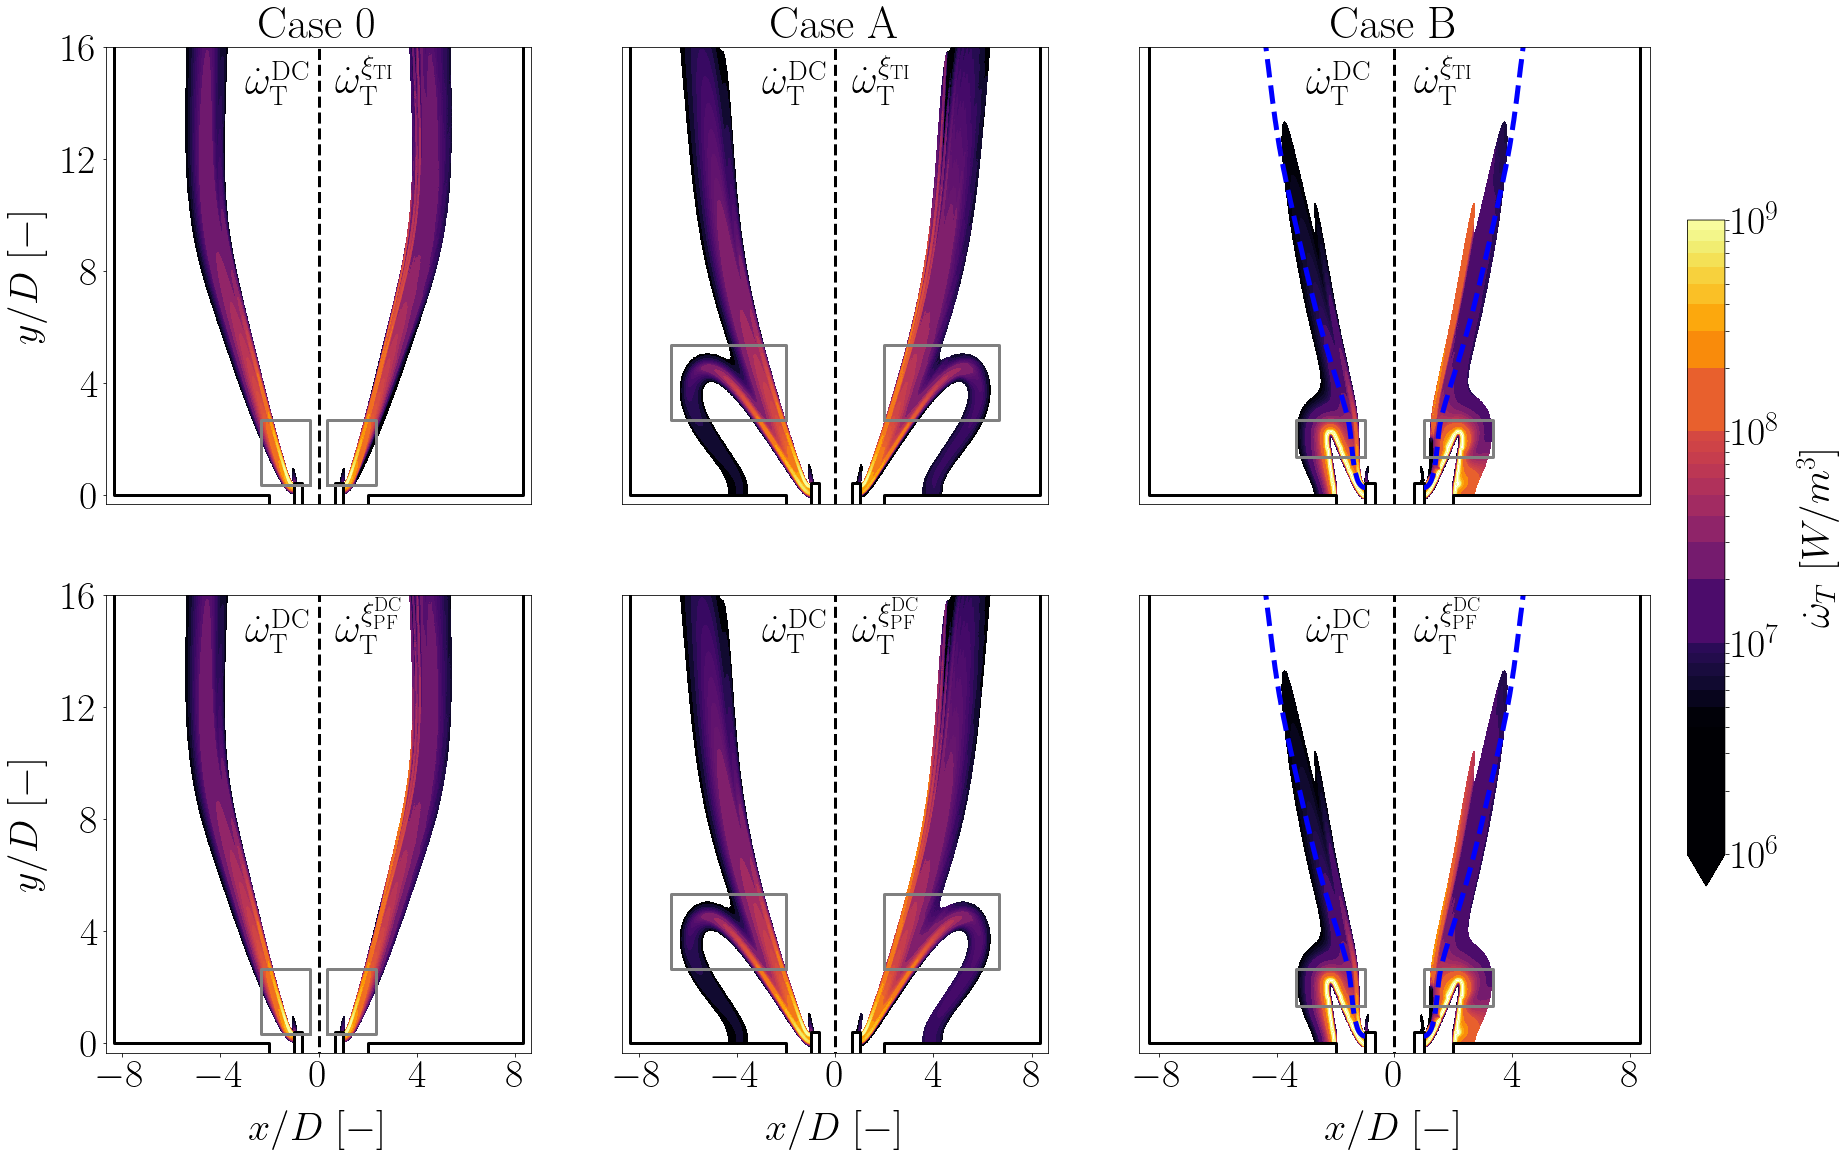
\includegraphics[scale=0.25]{./figures/FR_maps_a_priori_HRR}
    %\vspace{-0.5in}
	\caption{A-priori analysis of actual and reconstructed heat release fields for cases 0, A and B. The blue contour in case B corresponds to $Z = Z_\mathrm{st}$.}
	\label{fig:FR_maps_a_priori_HRR}
\end{figure}


A more quantitative description can be provided by plotting the three indices and heat release profiles along two different streamlines for case B. Fig.~\ref{fig:FR_Z_streamlines_plots} shows the mixture fraction distribution and two streamlines. Streamlines are born in the secondary inlet and then cross the perfectly premixed flame, denoted by the orange contours. The first streamline deviates towards the left side of the premixed flame and crosses the stoichiometric contour $Z = Z_\mathrm{st}$, while the second one deviates towards the right and stays in the lean region. Profiles are plotted along curvilinear coordinates $s_1$ and $s_2$, one per streamline. In the left streamline ($s_1$), all indices agree upstream. Beyond $s_1 > 2 D$, $\xi_\mathrm{TI}$ switches from diffusion to premixed detection, in contrast to $\xi_\mathrm{PF}$ which continues to detect diffusion in agreement with $\xi_\mathrm{id}$. Further downstream, $\xi_\mathrm{PF}$ starts to increase slowly for $s_1 > 6 D$, deviating from $\xi_\mathrm{id}$. This trend is also reflected in the heat release rate profiles, where the reconstructed rates accurately follow the DC trends up to $s_1 = 2 D$. Beyond that point, $\dot{\omega}_T^{\xi_\mathrm{TI}}$ shows a high rate corresponding to premixed conditions, while $\dot{\omega}_T^{\xi_\mathrm{TI}}$ identifies diffusion and the heat release is null, as in DC. For the right streamline ($s_2$), all indices agree in premixed combustion up to $s_2 = 2D$, where $\xi_\mathrm{id}$ plummets to 0, denoting non-premixed combustion. Scaled Takeno $\xi_\mathrm{TI}$ drops to $0$ further downstream at $s = 3D$, while $\xi_\mathrm{PF}^\mathrm{DC}$ smoothly decreases up to a value of $0.5$, disagreeing with the other two definitions. The reconstructed heat release rate profiles are identical to the DC upstream, retrieving the highest peak located at $s_2 = 2D$. Beyond this location, DC reduces up to $2 \cdot 10^6 ~ W/m^3$ while the reconstructed profiles stabilize both at $10^7 ~ W/m^3$. Even though the indices $\xi_\mathrm{TI}$ and $\xi_\mathrm{PF}^\mathrm{DC}$ differ for $s > 3D$, their corresponding heat release rates are identical. This is due to identical rates read from the diffusion and premixed flamelet tables at these locations, for which the heat release is underestimated with respect to DC. In spite of this, the peak and subsequent decreasing and stabilizing trend is properly recovered. 

Finally, temperature scatterplots in the mixture fraction space are shown in Fig.~\ref{fig:FR_scatterplots_a_priori}. They correspond to points within the spatial regions highlighted in gray in Fig.~\ref{fig:FR_maps_a_priori_HRR} for cases 0, A and B. $T^\mathrm{DC}$ correspond to the temperature directly obtained in the DC computations, while $T^{\xi_\mathrm{PF}^\mathrm{DC}}$ and $T^{\xi_\mathrm{TI}}$ correspond to temperature reconstructed from the indices as follows:

    \begin{equation}
    \label{eq:T_reconstr_PF}
    T^{\xi_\mathrm{PF}^\mathrm{DC}} = \xi_\mathrm{PF}^\mathrm{DC} \cdot  
    T^\mathrm{PTC} \left( Z, Y_c \right) + \left( 1 -  \xi_\mathrm{PF}^\mathrm{DC} \right) \cdot  T^\mathrm{DTC} \left( Z, Y_c \right), 
    \end{equation}


    \begin{equation}
    \label{eq:T_reconstr_TI}
    T^{\xi_\mathrm{TI}} = \xi_\mathrm{TI} \cdot  T^\mathrm{PTC} \left( Z, Y_c \right) + \left( 1 -  \xi_\mathrm{TI} \right) T^\mathrm{DTC} \left( Z, Y_c \right).
    \end{equation}

where $T^\mathrm{PTC}$ and $T^\mathrm{DTC}$ are the temperatures interpolated from the premixed and diffusion manifolds, respectively. In general, the reconstructed temperatures recover the same trends and values from the DC computation. Deviations are found in the rich region of case 0. In the former, temperature is slightly underestimated at $Z \sim 0.2$ for $T^{\xi_\mathrm{PF}^\mathrm{DC}}$, while $T^{\xi_\mathrm{TI}}$ shows even lower values for $0.2 < Z < 0.4$. In the region of case A, the predicted values are accurate for the entire mixture fraction range. Finally, for case B, there are mispredictions in the leanest regions close to the lower flammability limit, while deviations are also observed in the richest cases where there is a higher dispersion of both $T^{\xi_\mathrm{PF}^\mathrm{DC}}$ and $T^{\xi_\mathrm{TI}}$ compared to $T^\mathrm{DC}$. Nevertheless, the reconstructed temperatures at these locations match between themselves, suggesting that the interpolated temperatures $T^\mathrm{PTC}$ and $T^\mathrm{DTC}$ are identical at this location and underestimate the temperature from DC, similarly to what ocurred in the second streamline of Fig.~\ref{fig:FR_Z_streamlines_plots}.

Overall, this section has shown through an \textsl{a-priori} analysis that reconstructing reactive fields through the premixedness index $\xi_\mathrm{PF}$ can recover the properties from a DC computation without assumptions on the burning regimes. These reconstructed fields are in line with the predictions from the Takeno index $\xi_\mathrm{TI}$, \textbf{sometimes even improving those}. The next step is to evaluate the capability of $\xi_\mathrm{PF}$ to blend premixed and diffusion manifolds in CFD simulations during runtime, which is done in the following section.

%\begin{figure}[h!]
%    \centering
%	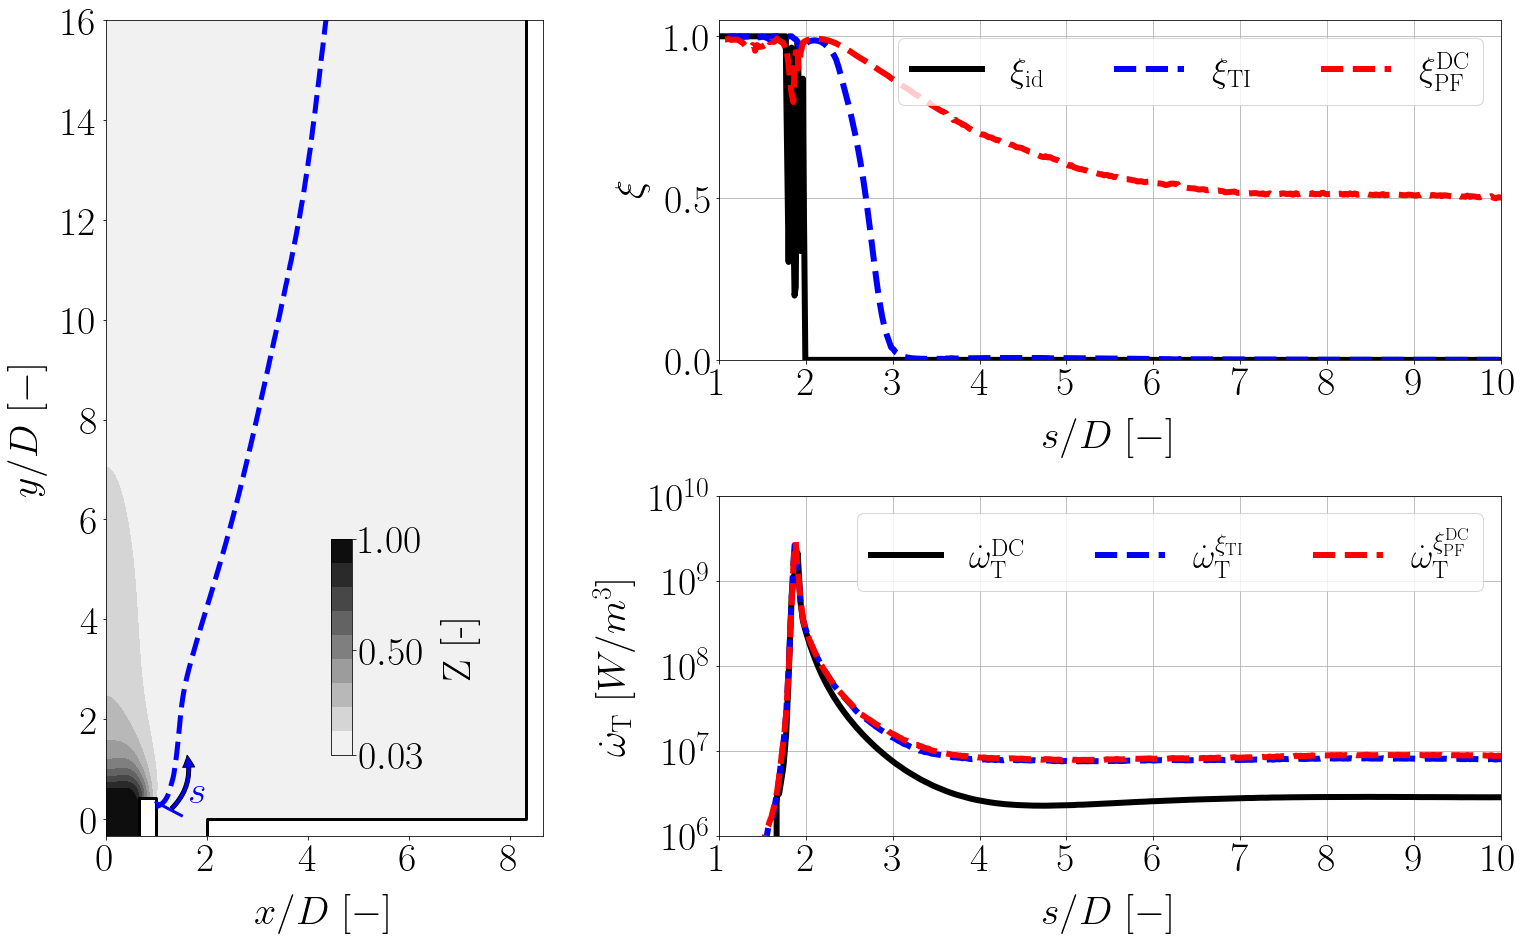
\includegraphics[scale=0.15]{./figures/FR_Z_contour_plots}
    %\vspace{-0.5in}
%	 \caption{Mixture fraction distribution in case B. The $Z_\mathrm{st}$ contour is represented by the dashed blue line. Profiles of flame indices and heat release are shown along the stoichiometric line. \textbf{THIS SHALL BE REMOVED}}
%	\label{fig:FR_Z_contour_plots}
%\end{figure}

\begin{figure}[h!]
    \centering
	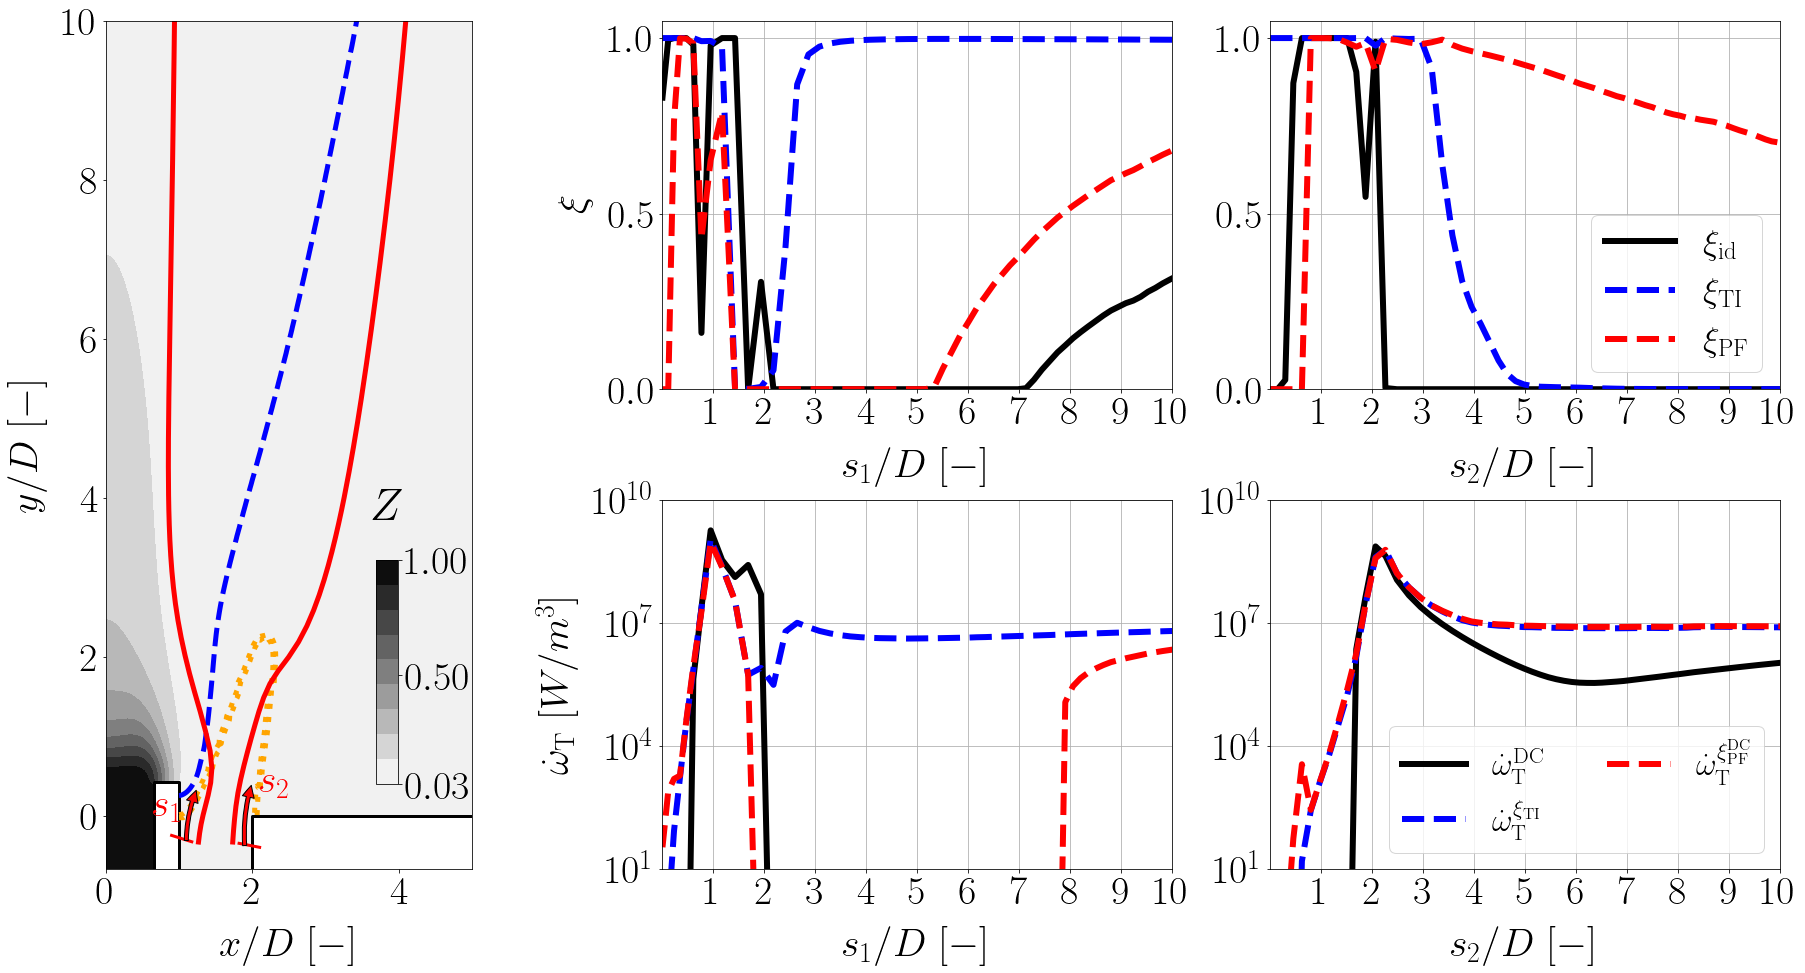
\includegraphics[scale=0.22]{./figures/FR_Z_streamlines_plots}
    %\vspace{-0.5in}
	\caption{Mixture fraction distribution in case B (\textsl{left}). The red lines represent two streamlines along which the flame indices and heat release rates are represented in the middle and right rows. The blue line denotes the isoline $Z_\mathrm{st}$. The orange contour represents the perfectly premixed flame.}
	\label{fig:FR_Z_streamlines_plots}
\end{figure}


\begin{figure}[h!]
    \centering
	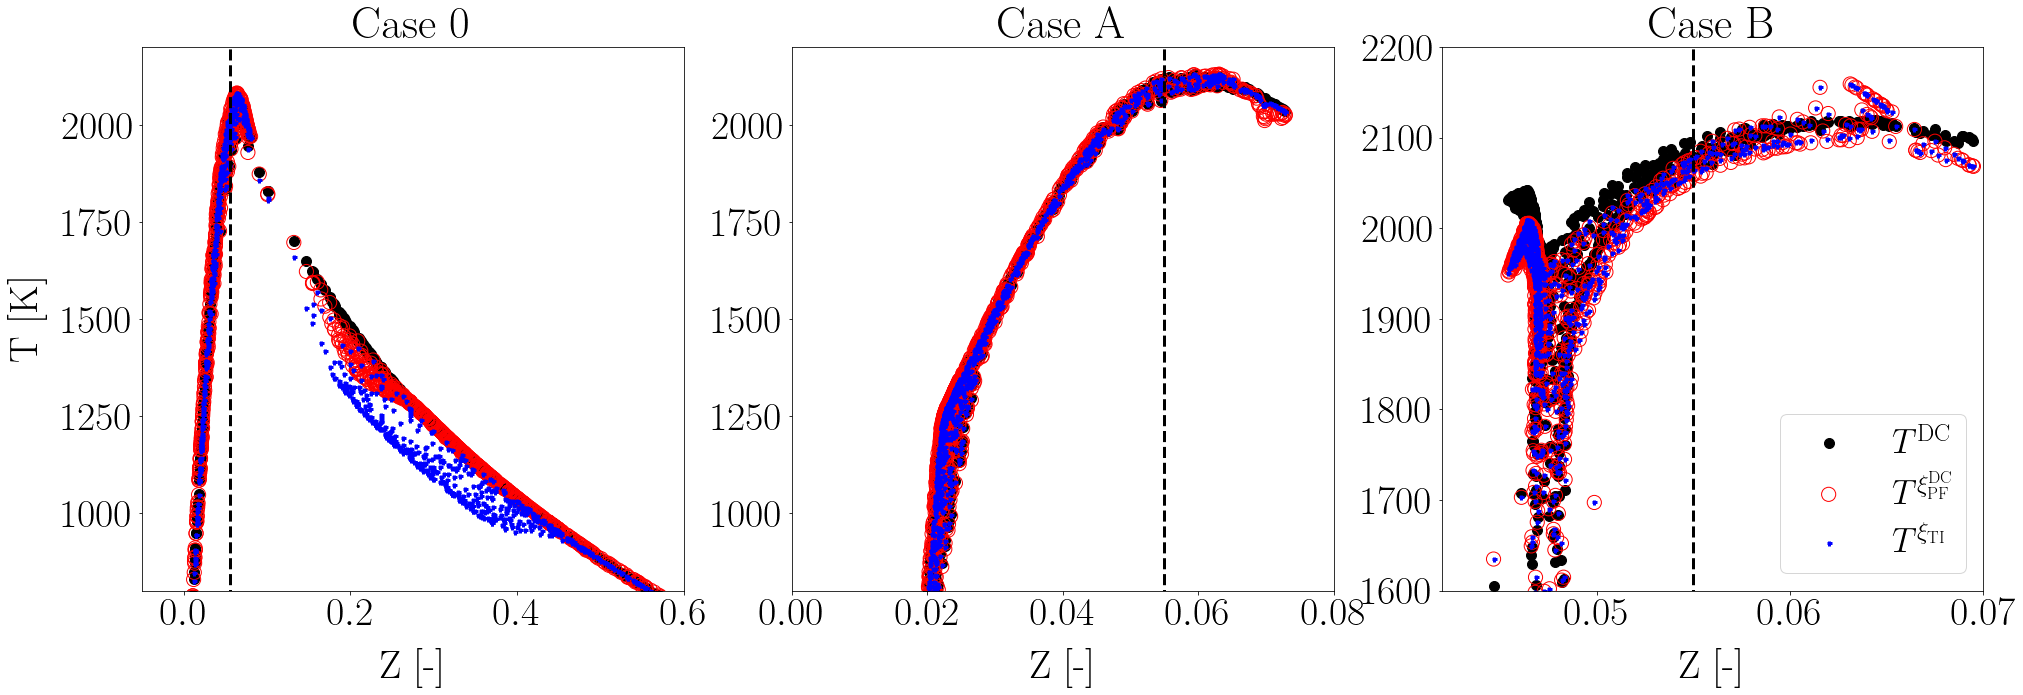
\includegraphics[scale=0.2]{./figures/FR_scatterplots_a_priori}
    %\vspace{-0.5in}
	\caption{Temperature scatterplots in the $Z$ space for points within the spatial regions in grey from Figure \ref{fig:FR_maps_a_priori_HRR}. The black dashed line denotes the stoichiometric mixture fraction.}
	\label{fig:FR_scatterplots_a_priori}
\end{figure}

\clearpage


\subsection{A posteriori analysis}
\label{subsec:fts-a-posteriori}



The assessment of the proposed flamelet-based premixedness index is extended here for \textsl{a posteriori} analysis using the cases presented in Table~\ref{tab:BCs_simulations}. The analysis includes the solution fields obtained from the use of premixed flamelets (PTC), diffusion flamelets (DTC) along with the results of the premixedness index (TC). 

\dmm{

\textsl{LETS COMPLETE THIS PARAGRAPH ONCE THE RESULTS ARE DONE}
}

\subsubsection{Flow fields and thermal states}


The flow fields and thermal states of the five distinct cases is analysed here for the different tabulated flamelet approaches. Results of these methods for the temperature field are shown in Fig.~\ref{fig:fts_maps_comparison_T_flamelets_FR} for comparison. \dmm{Note the velocity and mixture fraction fields are rather similar for all the cases, so they are omitted for the sake of brevity } \textbf{ACTUALLY NOT}. \textbf{CHECK NEXT PARAGRAPH AND PUT IT HERE WHEN READY}

The plots of temperature demonstrate that the proposed flamelet index effectively captures the flame topology qualitatively across all cases, representing the spatial distribution, temperature values, and flame structure. It successfully predicts the shape and length of the premixed flames in Cases B and C, as well as identifying the non-reactive regions formed by the coflow stream in Cases 0, A, and D, where a non-flammable mixture is injected. \textbf{In Cases 0, A, and B, discrepancies appear near the centerline, where the TC model underestimates the temperature compared to DC results} (\textbf{THIS SHOULD BE CHANGED ONCE RESULTS ARE UPDATED}). The highest temperatures in these cases are observed in the diffusion branch, aligning well with the expected diffusion flamelet solutions. Case C, in particular, exhibits higher temperatures at the interface between the central and outer mixtures, consistent with the diffusion regime, while further radially, the behavior transitions to a premixed-like manifold. For Cases B and D, the flame index accurately retrieves the shape of the premixed flame, capturing the flame length with a slight underestimation compared to the diffusion manifold. 

\dmm{\textsl{WE SHOULD DISCUSS THE T FIELDS FOR THE DIFFERENT METHODS HERE AS WELL, NOT ONLY THE INDEX}}

%Overall, the flame index provides a robust approximation of the flame characteristics across both premixed and diffusion combustion regimes, maintaining accuracy in temperature prediction and flame topology.

%The temperature fields show that the proposed flamelet index can recover the flame topology featured by the different cases. The results indicate the use of the flame index  represents accurately the spatial distributions and values of the DC, as well as the shape and length of the premixed flames featured in Cases B and C, as well as the non-reactive branches outside the main injector in cases 0, A and D (where a non-flammable mixture is injected). Disagreements are found in the region around the centerline in cases 0, A and B, where TC underestimates the temperature with respect to DC. Cases 0, A and B present the highest temperatures in the diffusion branch which matches the values and shape from the diffusion flamelet solutions. Case C shows higher temperatures in the lip between the central and outer mixture that match the diffusion case, while further radially the regimes corresponds to that of premixed manifold. In cases B and D, the most significant feature is the shape of the premixed flame, which the flame index retrieves the length of the premixed case, though slightly shorter than the diffusion computation.






\begin{figure}[h!]
\centering	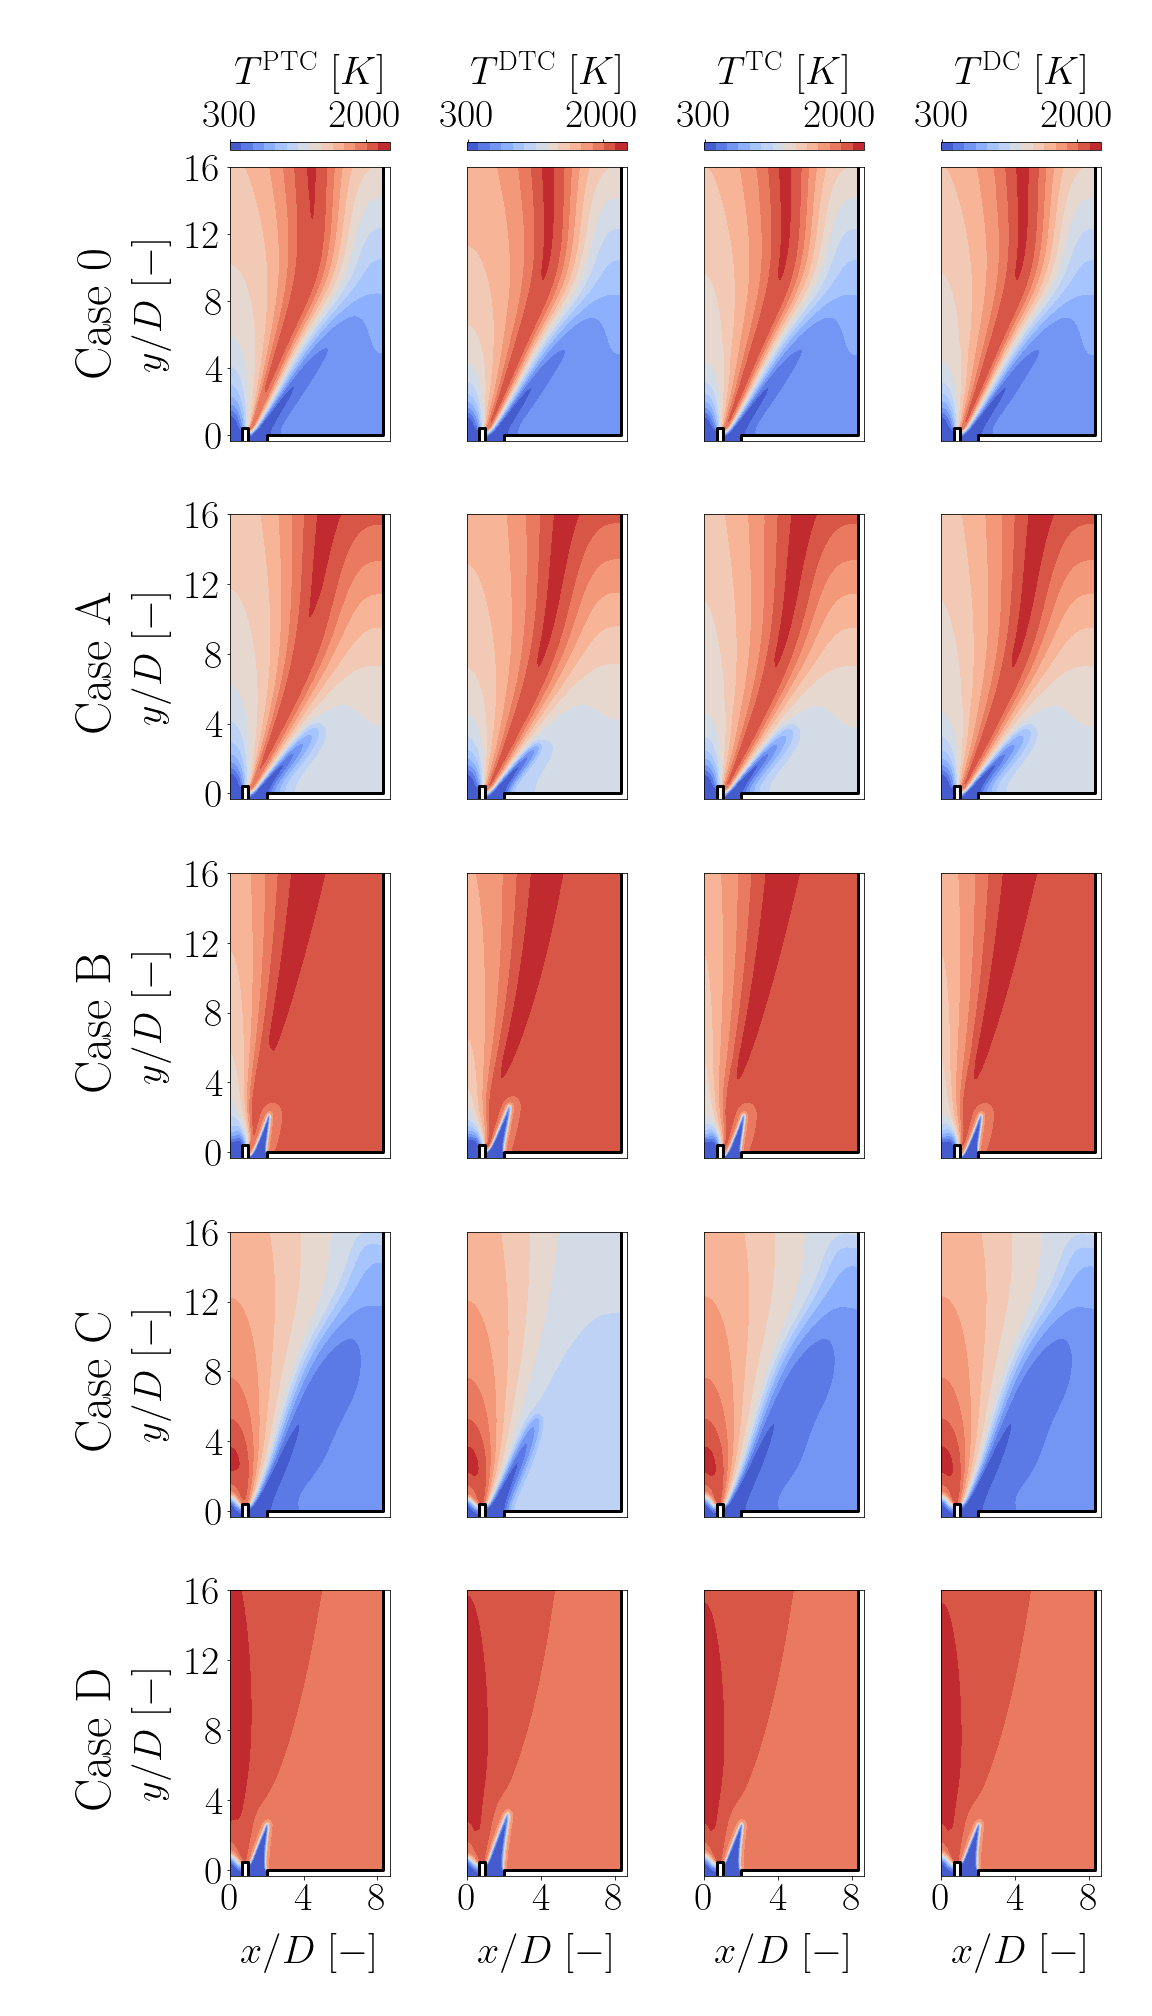
\includegraphics[scale=0.25]{./figures/fts_maps_comparison_T_flamelets_FR}
    %\vspace{-0.5in}
	\caption{Temperature fields for simulations of individual flamelets (PTC, DTC), blended multiregime flamelets (TC) and Direct Chemistry (DC).}
	\label{fig:fts_maps_comparison_T_flamelets_FR}
\end{figure}



\clearpage




Further insights into the temperature field can be gained by examining radial profiles at two different axial distances, given in Fig.~\ref{fig:fts_profiles_T_all}. DC solutions are compared to the complete set of flamelets computations (PTC, DTC and TC). In all cases, the flame index case lies within the limits of premixed and diffusion flamelet manifolds. Improvements with respect to individual flamelets computations are observed in most cases. An case A, the TC approaches the FR simulation in all the radial axis at $y/D = 1.5$, from the centerline, where diffusion is identified up to $x/D \sim 3$, and outwards, where premixedness is identified for $x/D > 3$. All cases show a similar behavior, with the flame index outperforming premixed and diffusion flamelets. Deviations are found close to the centerline in cases 0, A and B, which is specially relevant further downstream at $y/D = 6.5$. Here, the blended TC computation retrieves a value between premixed and diffusion flamelets, in most cases closer to pure premixedness, while the diffusion flamelet simulation is the one which better approaches the DC case. This suggests that the central region corresponds to a diffusion region, which the premixedness index is unable to capture. Indeed, reaction rates in this area are low, as will be shown in Figure \ref{fig:fts_maps_indicees_comparison}, where the white regions denote regions of low or null reactivity. Therefore, the gradient of progress variable is low or close to $0$ in this area, and the index $\xi_\mathrm{PF}$ provides a value close to $1$ (pure premixedness) given that $k = 1$ (i.e. the mixture is within the flammability limits) according to Eq. (\ref{eq:zeta_PF_illana}). As a result, $\xi_\mathrm{PF}$ identifies premixed-like combustion when indeed diffusion flamelets retrieve better the DC works. This is a limitation of the model to recover the asymptotic limit of non-premixed combustion, though overall provides an improved performance compared to the premixed flamelet manifold. 

\dmm{\emph{WE SHOULD DISCUSS THIS POINT MORE CAREFULLY HERE. BUT BEFORE THIS, WE SHOULD HIGHLIGHT THE GOOD ASPECTS OF THE METHOD, HIGHLIGHTING ALSO THE ABILITY OF PTC TO PREDICT THESE FLOW CONDITIONS AND THE LIMITATION TO RECOVER THE DIFFUSION LIMIT TO EXPOSE THE BENEFIT OF USING OUR APPROACH -- @Anurag: can you revise this part?}}

%of the present model that will be targeted in future works.

\begin{figure}[h!]
        \centering
	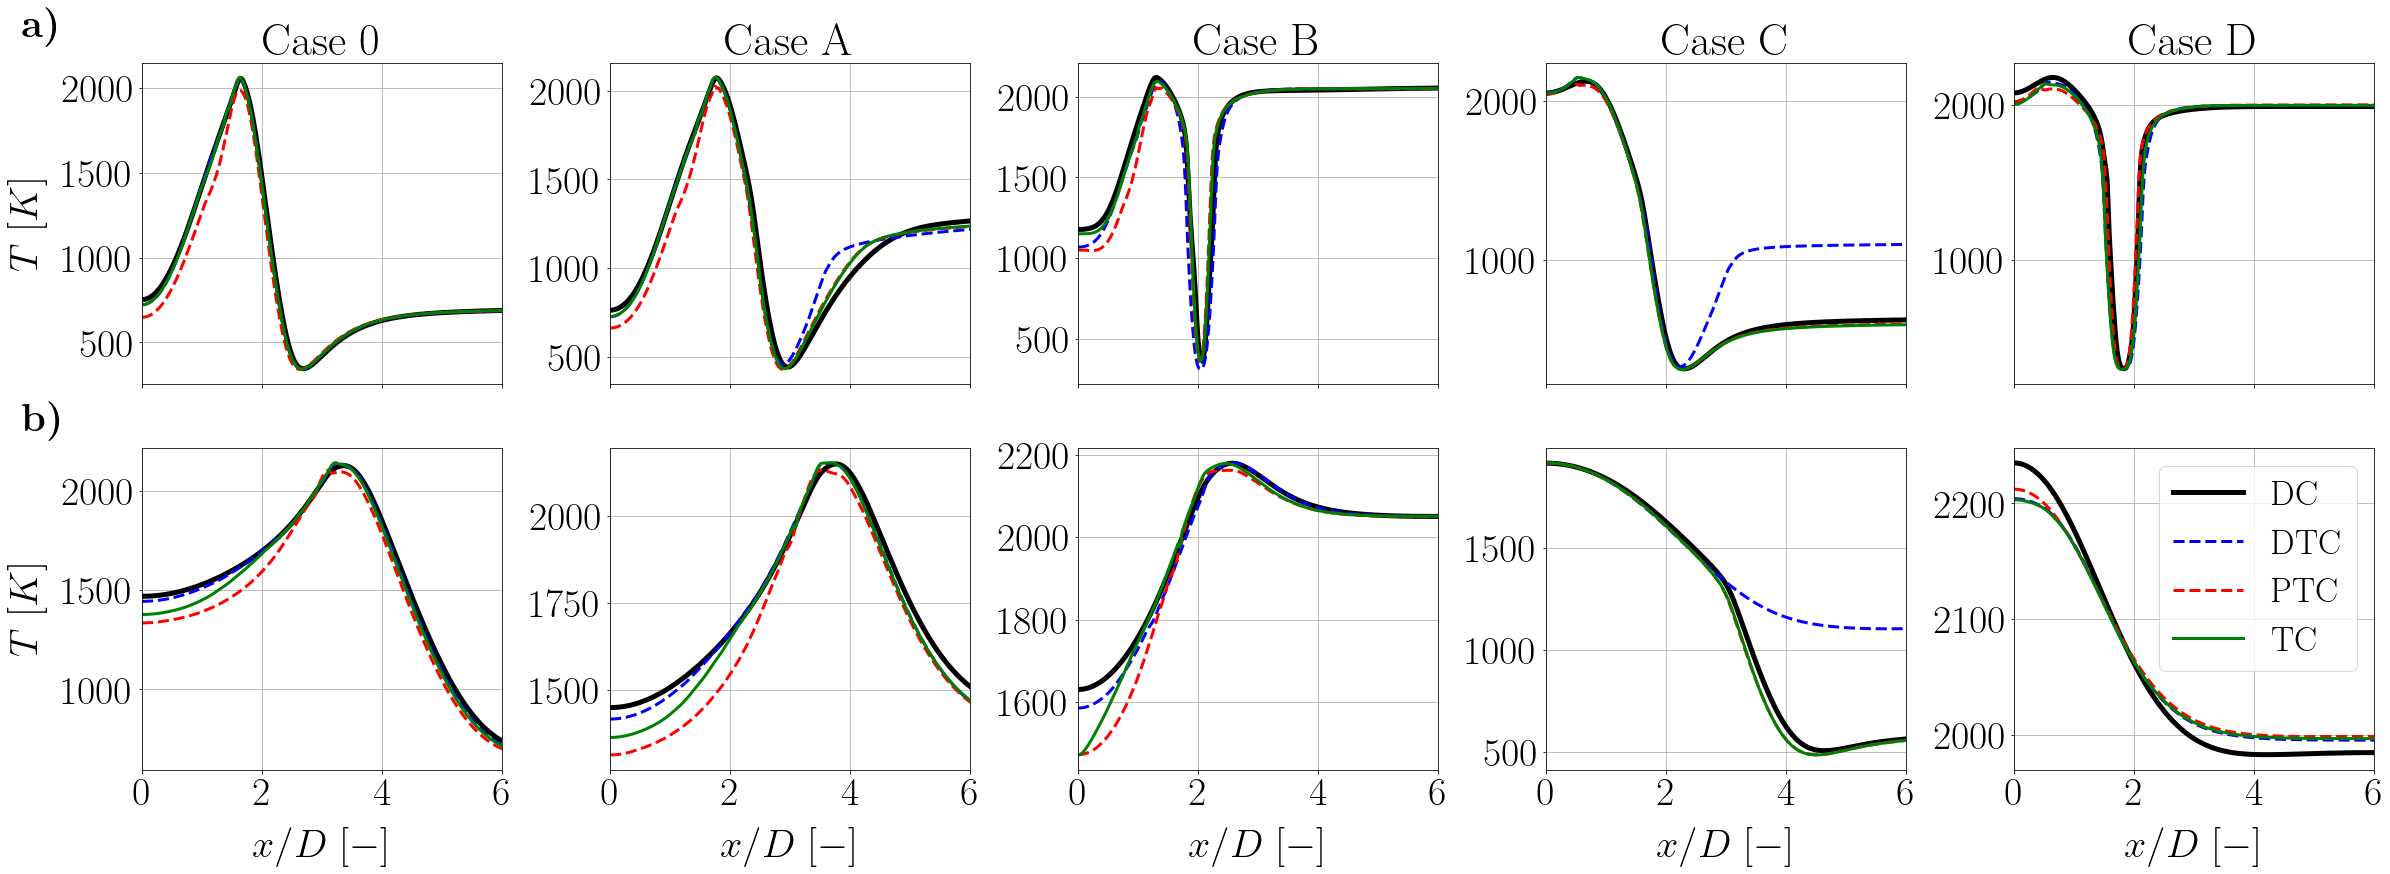
\includegraphics[scale=0.16]{./figures/fts_profiles_T}
	\caption{Temperature profiles along lines at a) $y/D = 1.5$, b) $y/D = 6.5$.}
	\label{fig:fts_profiles_T_all}
\end{figure}

Further comparisons between the flame index solutions with the detailed chemistry are shown
%DC and TC with the multiregime model are compared 
in Fig.~\ref{fig:fts_maps_OH_CO_CO2}, where species mass fractions (OH, CO, CO$_2$) are visualized. Species agreement between both cases is generally good, specially for OH and CO$_2$. More discrepancies are found for CO, where TC overestimates this quantity in cases 0, A and B. This overestimation of CO is in agreement with the results of \cite{illana_extended_2021} for partially-premixed counterflow flames: it is attributed to the definition used for the progress variable, which is identical in both works. Species predictions could be improved by using flamelet libraries with different progress variable definitions \citep{both_high-fidelity_2023}, or by resolving additional transport equations for such species \citep{massey_large_2023}. 



\begin{figure}[h!]
\centering
	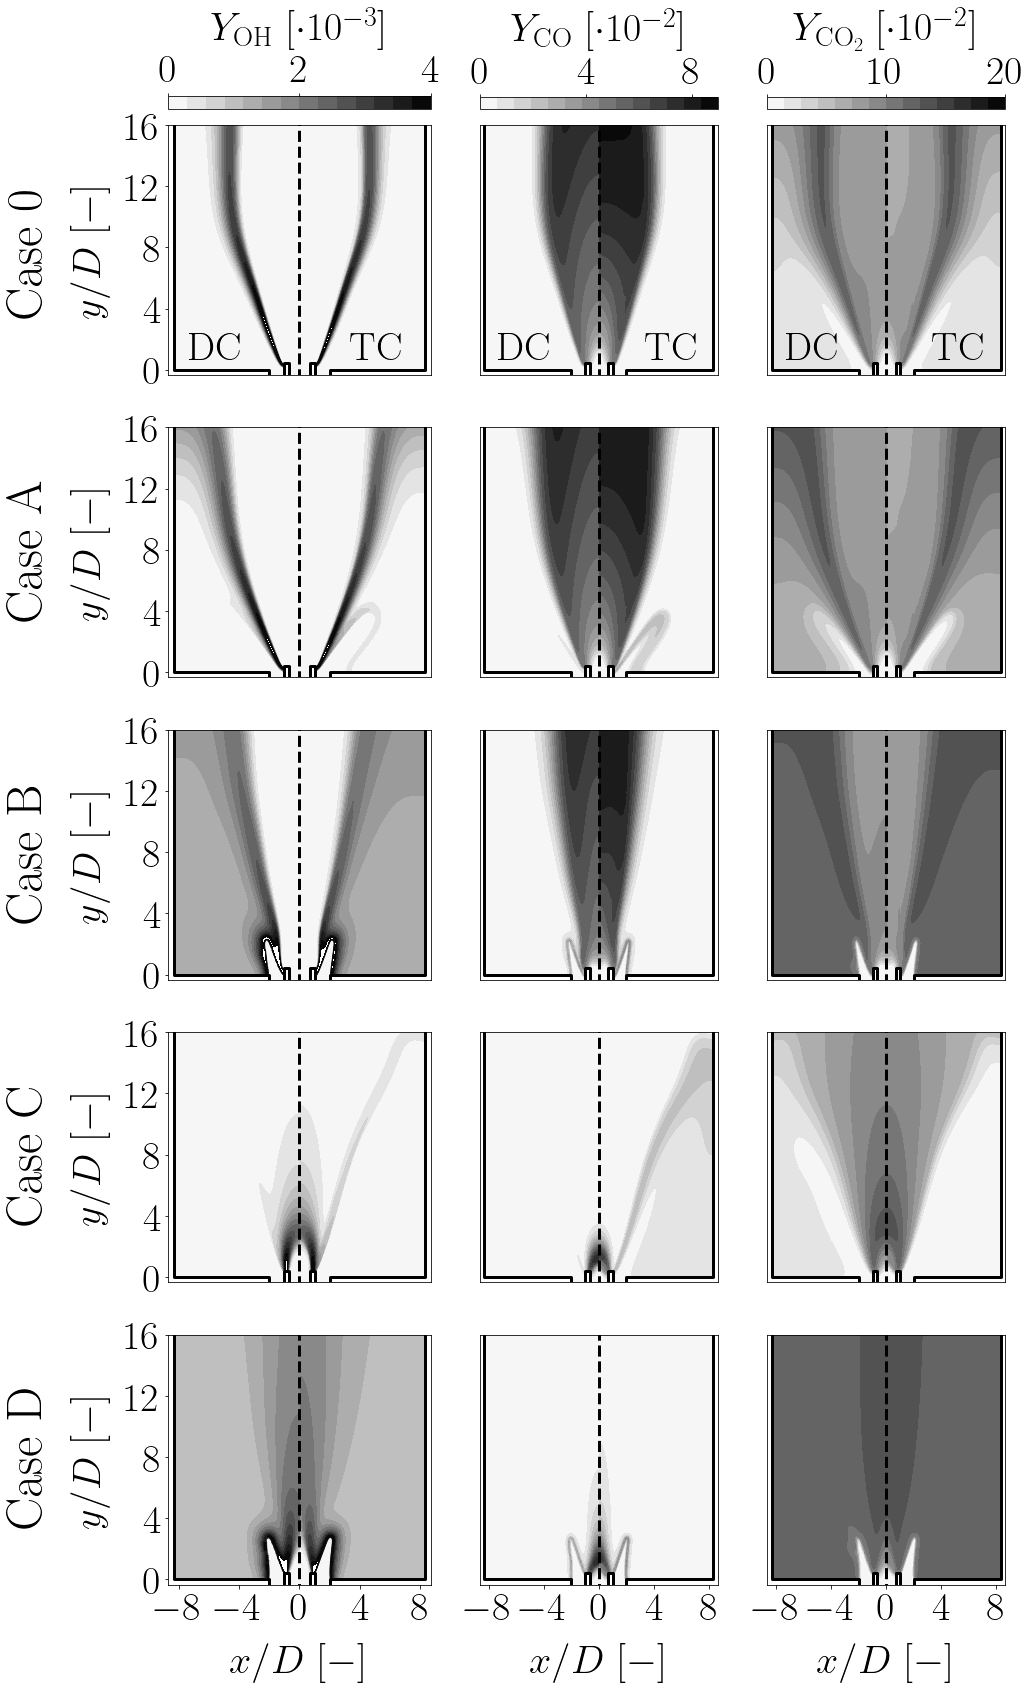
\includegraphics[scale=0.25]{./figures/fts_maps_OH_CO_CO2}
    %\vspace{-0.5in}
	\caption{Species from flamelet computations with TC compared to DC.}
	\label{fig:fts_maps_OH_CO_CO2}
\end{figure}




\clearpage


along with the premixedness index $\xi_\mathrm{PF}$. Using the $\xi_\mathrm{PF}$ index as a marker of multiregime phenomena due to its ability to discriminate these regions, as shown in the previous sub-section, the plots show that the different cases present co-existence of premixed- and diffusion-dominated fronts, except for Case 0 (pure diffusion flame). Premixedness levels then increase from cases A to D,
where the incoming mixture on the coflow jet is enriched from lean to rich conditions. 


%values comprised between the premixed and diffusion flamelets, averaged according to the value of index $\xi_\mathrm{PF}$. 


\subsubsection{Multiregime phenomena}

Further analysis of the ability of the premixed index to predict multiregime phenomena is discussed here. The premixedness index $\xi_\mathrm{PF}$ is now compared to the Takeno index $\xi_\mathrm{TI}$ obtained from the DC solutions in Figure
\ref{fig:fts_maps_indicees_comparison}, where only regions with significant heat release are retained to aid the comparisons. As opposed to the Takeno index, $\xi_\mathrm{PF}$ shows a smooth transition between premixed and diffusion modes, as previously shown in the \textsl{a priori} analysis. In Cases A, B and D, with high heat release outside the outer injector, both indices agree on premixed combustion mode. In the diffusion branches of cases 0 and A, Takeno predicts diffusion closer to the centerline and premixedness further radially, while the premixedness index predicts pure diffusion highlighting its ability to capture diffusion-dominated conditions. Discrepancies are also found for Case C, where the TC solution retains the use of the diffusion manifold as compared with the Takeno index. \dmm{\emph{WHAT IS THE BEHAVIOUR OF THE IDEAL INDEX HERE? WE SHOULD RELATE IT HERE}}
%indicates a higher prevalence of diffusion than the DC simulation evaluated with the Takeno index. 
%Overall, the premixedness index $\xi_\mathrm{PF}$ 
%applied to flamelets computation 
%identifies more diffusion-dominated regions than the Takeno is used for evaluation in the DC cases, as also observed previously when $\xi_\mathrm{PF}^\mathrm{DC}$ was applied \textsl{a priori} to postprocess DC results.

\begin{figure}[h!]
\centering
	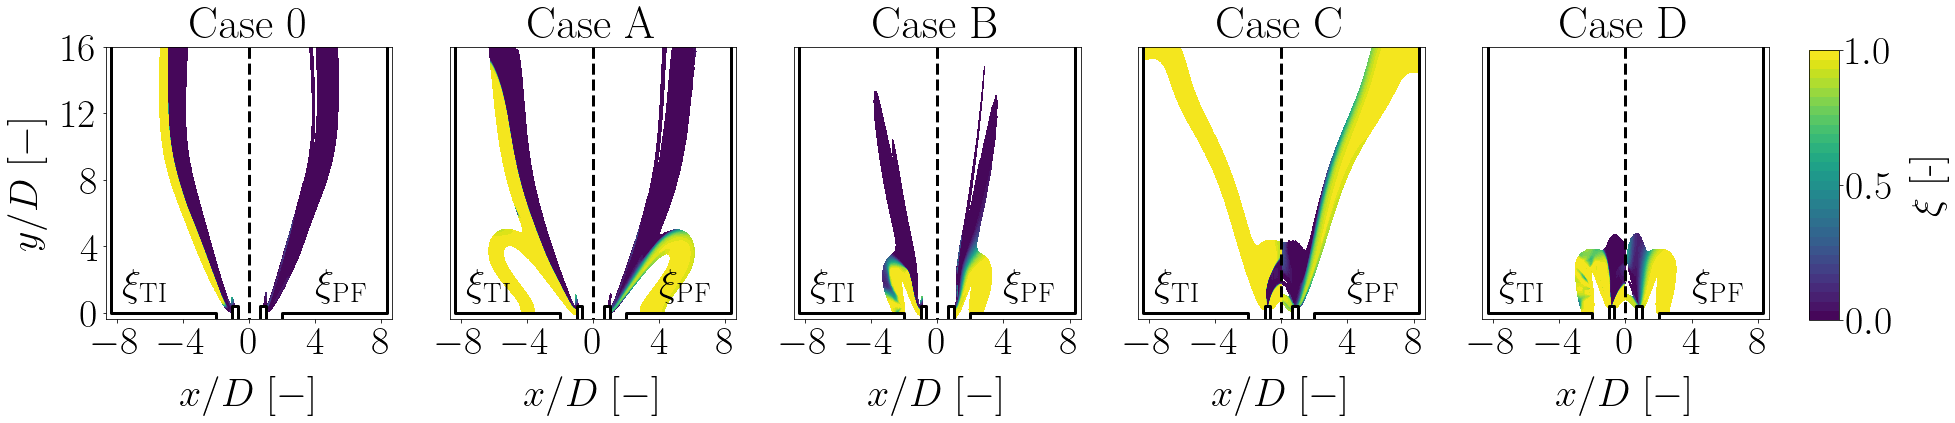
\includegraphics[scale=0.21]{./figures/fts_maps_indicees_comparison}
    %\vspace{-0.5in}
	\caption{Comparison of flame indices, shown at the regions where the heat release rate $\dot{\omega}_T$ is larger than $0.1~\%$ of the maximum value in each case.}
	\label{fig:fts_maps_indicees_comparison}
\end{figure}


Heat release rate for the high reactive regions in three cases are now shown in Fig.~\ref{fig:fts_maps_a_posteriori_HRR} for comparison. Results from the flame index calculation 
%with the multiregime model 
are represented against the DC in the first row, and 
%against 
the \textsl{a priori} reconstructed fields with $\xi_\mathrm{PF}^\mathrm{DC}$ in the second row. Comparison with DC shows that the TC computation recovers accurately the reaction rates from the table. Disagreement appears for Case A in the outwards region close to the secondary injector, where heat release is overpredicted. This characteristic is not present in the reconstructed heat release shown in the second row. Nevertheless, in that case the reconstructed field overpredicts the heat release in the inner part of the diffusion branch downstream the injectors, while the TC computation predicts properly this quantity when compared to DC. 


\begin{figure}[t!]
        \centering
	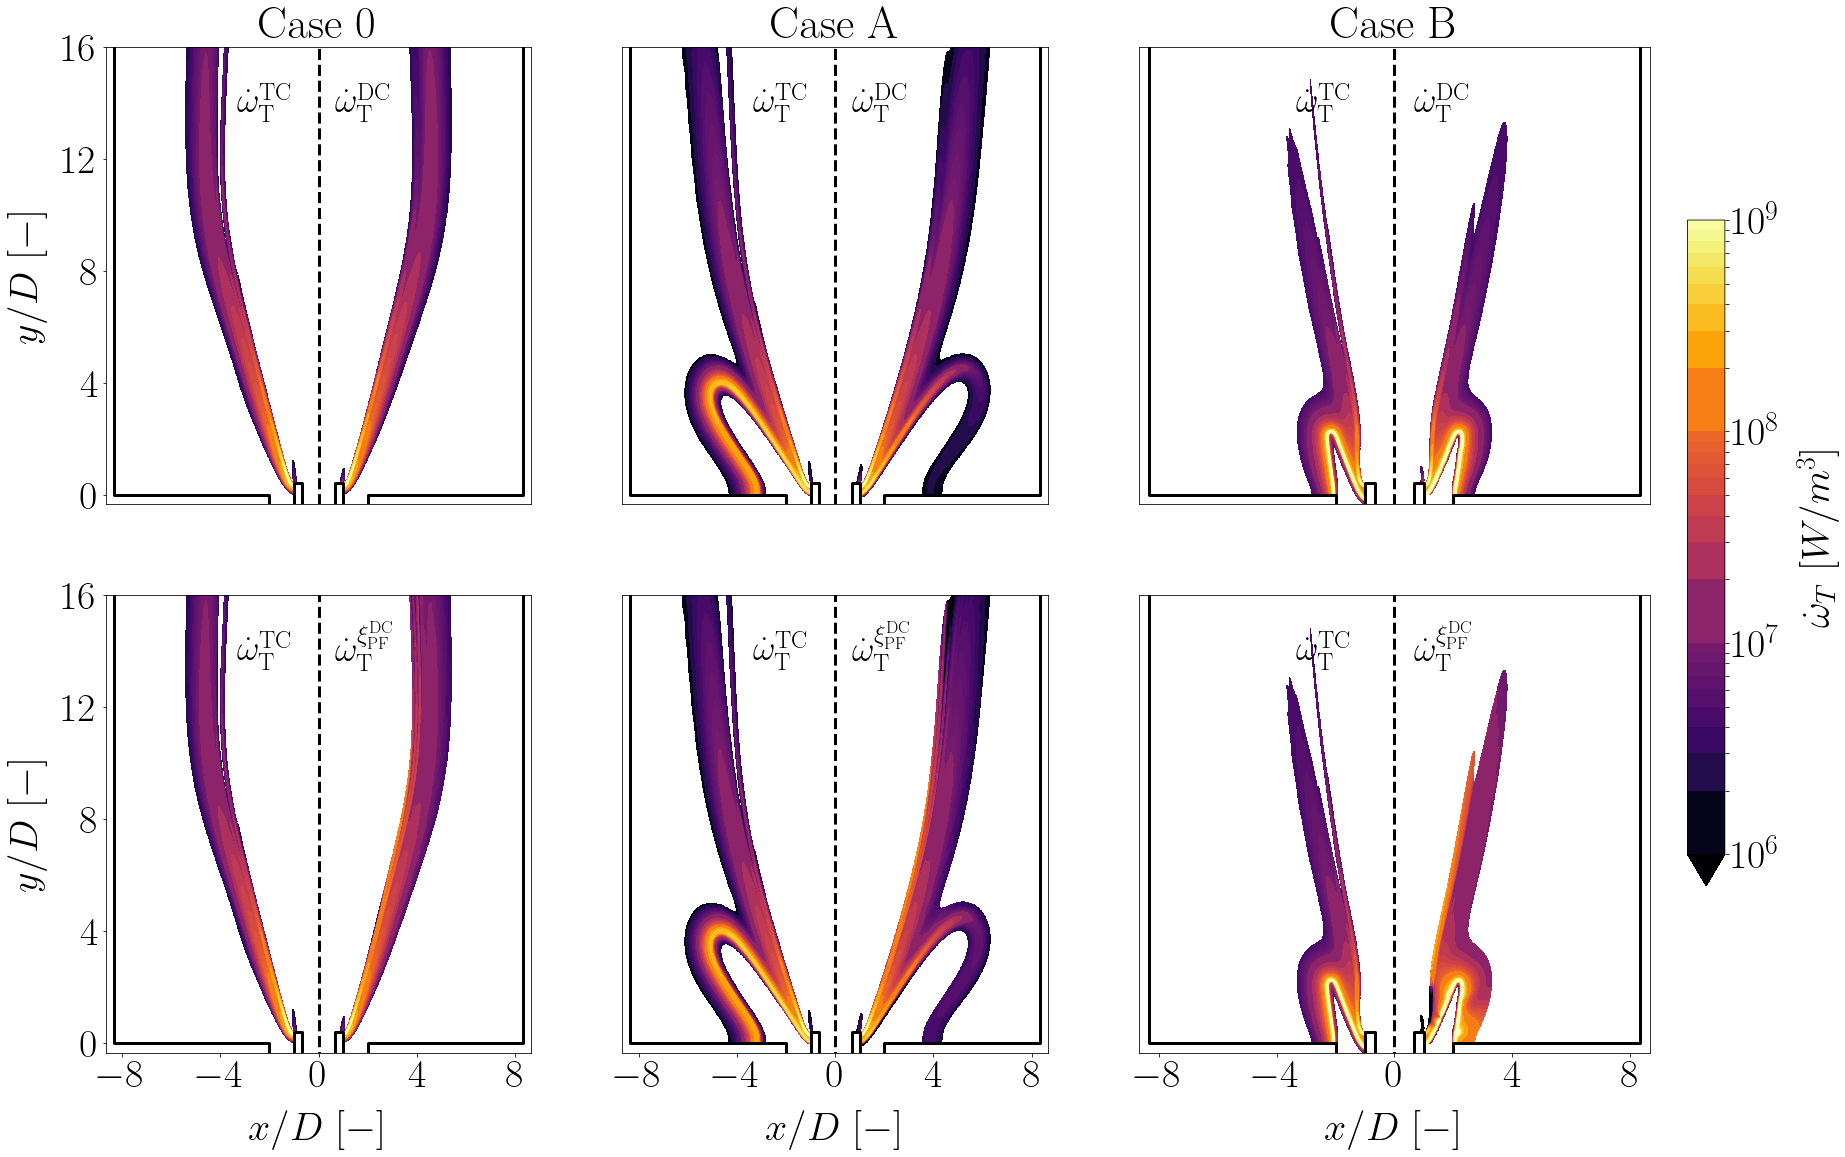
\includegraphics[scale=0.22]{./figures/fts_maps_a_posteriori_HRR_2rows}
    %\vspace{-0.5in}
	\caption{Heat release fields for TC, DC and \textsl{a-priori}  $\xi_\mathrm{PF}$ reconstructed heat release rate fields from the Takeno and premixedness indices. }
	\label{fig:fts_maps_a_posteriori_HRR}
\end{figure}

A quantitative view of the heat release is given by plotting radial profiles for Case B at two axial distances ($y/D = 1.5, 6.5$) in Fig.~\ref{fig:HRR_profiles_a_posteriori}. DC and TC results are plotted together with the \textsl{a-priori} reconstructed fields from the indices $\xi_\mathrm{TI}$ and $\xi_\mathrm{PF}$. The use of the premixed index
%computation where the index 
$\xi_\mathrm{PF}$ 
%is used to merge flamelet manifolds 
yields better results than when interpolated the solutions as shown in the\textsl{a priori} tests. Closer to the injectors ($y/D = 1.5$), all lines follow a similar behaviour to DC. Further downstream ($y/D = 6.5$), the TC captures accurately the low reactivity of the DC computation, while the reconstructed fields overestimate heat release with peaks located at $x/D \sim 2$. These results show that the \textsl{a priori} reconstructed indices provide an estimation of the heat release fields, but their performance is always worse than when the premixedness index is applied \textsl{a posteriori} during runtime, yielding results that approach the DC simulation but with lower computational cost (\textbf{quantify this time reduction!}). 
%Therefore, this proves the ability of the studied methodology to simulate partially premixed conditions close to real systems with a tabulated chemistry methodology based on flamelets.
These results prove that the $\xi_\mathrm{PF}$ index is able to recover the heat release rate and the associated thermal states for conditions involving stratification and transitions between diffusion and premixed flames. 

\begin{figure}[h!]
    \begin{subfigure}[b]{0.45\textwidth}
        \centering
        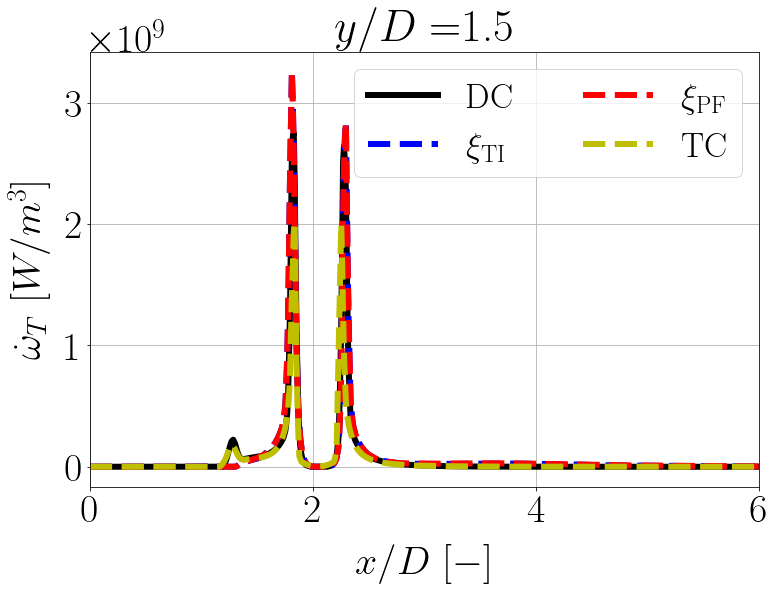
\includegraphics[scale=0.24]{./figures/profiles_a_posteriori/profile_y_5mm}
    \end{subfigure}
    %\hfill
    \hspace{0.45in}
    \begin{subfigure}[b]{0.45\textwidth}
        \centering
        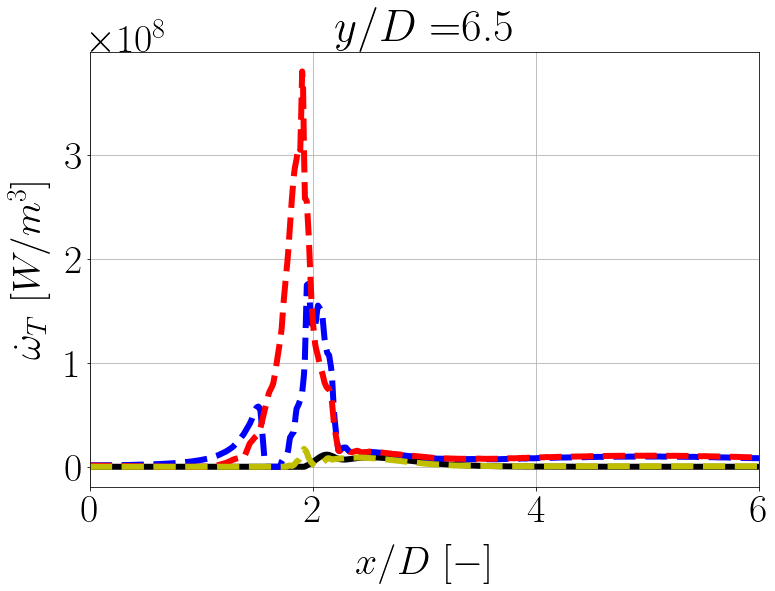
\includegraphics[scale=0.24]{./figures/profiles_a_posteriori/profile_y_20mm}
    \end{subfigure}
    %\hfill
	\caption{Radial profiles of heat release rate for Case B.}
	\label{fig:HRR_profiles_a_posteriori}
\end{figure}

\subsubsection{Flame structure}

Finally, an analysis of the flame structure is presented with the aim to evaluate the predictive capability of the model to recover the production of major species and radicals. Cases A and B are selected for this analysis, as those represent well the existence of multiregime phenomena in this configuration. In particular, two regions located across the transitions from the central flame and the flame stabilized over the coflow mixture are selected for the analysis, see Fig.\ref{fig:fts_scatterplots_maps_regions}. The field $\xi_\mathrm{PF}$ shows that both regions contain a stratified mixture. The region I corresponds to the near field of the flame exiting the coflow where the flame attaches to the burner, while region II corresponds to reacting layer formed by the diffusion flame of the central injection with the coflow mixture. 


\begin{figure}[h!]
    \centering
	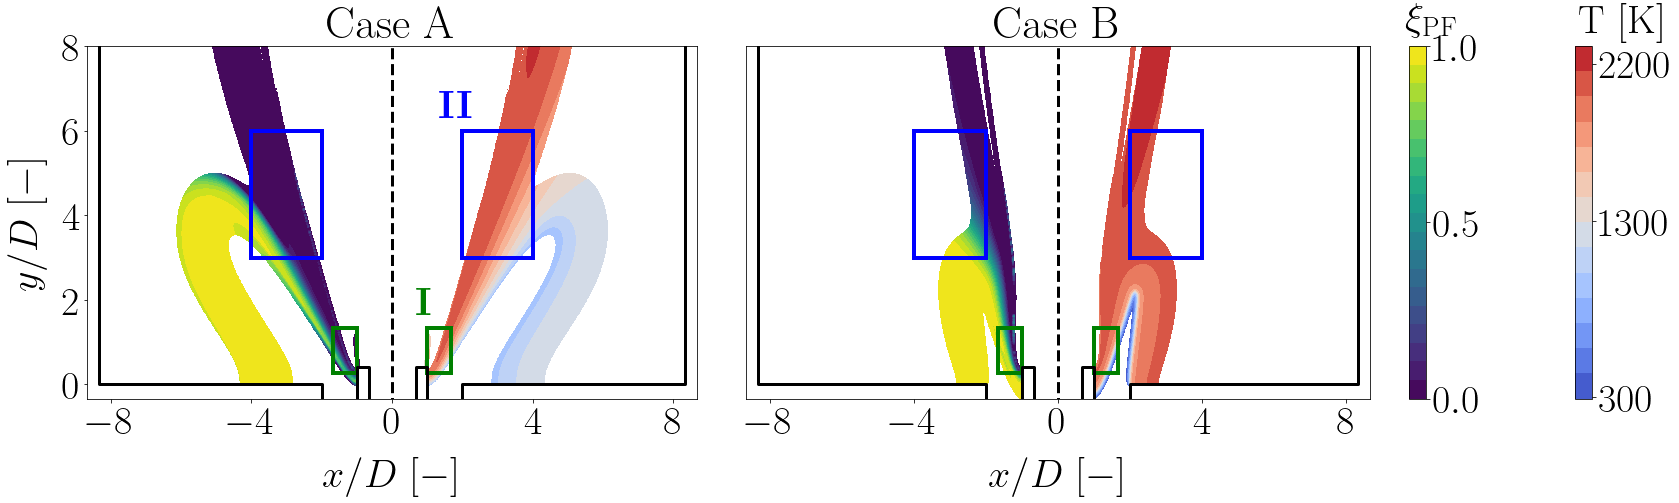
\includegraphics[scale=0.225]{./figures/fts_scatterplots_maps_regions}
    %\vspace{-0.5in}
	\caption{Fields of index $\xi_\mathrm{PF}$ and temperature for cases A and B shown at regions of high heat release for the TC simulation. The squares indicate regions I and II where point data are analyzed.}
	\label{fig:fts_scatterplots_maps_regions}
\end{figure}

The flame structure is analysed by using conditional means of temperature and mass fractions (OH, CO, CO$_2$) to the mixture fraction 
for the regions I and II. The conditional mean is computed for the points within each region where $\dot{\omega}_T$ is larger than the $0.1~\%$ of the maximum value from $\dot{\omega}_{T}^\mathrm{DC}$. The data is grouped into bins of size $\Delta Z = 2 \cdot 10^{-3}$ intervals along the mixture fraction axis, and then the average within each bin is calculated. The different plots for region I and II are shown in Figs.~\ref{fig:fts_scatterplots_lines_A2} and \ref{fig:fts_scatterplots_lines_A7} respectively. 
The results for region I show the flame index 
reproduces fairly well the reference DC results for all magnitudes. Exceptions are observed for Case A at lean conditions, where TC overestimates the mass fraction of CO as it follows the diffusion limit. This is a well-known effect~\cite{illana_extended_2021,fiorina_approximating_2005,zirwes_identification_2021} since CO cannot be represented by the
two asymptotic limits of combustion and requires a more dedicated closure, which is out of the scope of the present work. 
%while it is the premixed flamelets computation the one that best approaches the finite rate. 
Similar observations can be obtained for region II, as observed in Fig.~\ref{fig:fts_scatterplots_lines_A7}, where in this case the flame index approaches the DC in all plots. Altogether, while discrepancies are observed for the PTC and DTC flamelet computations with respect to DC, the blending these manifolds with the proposed index $\xi_\mathrm{PF}$ is shown to substantially improve the predictions of the major species and the OH radical with respect to the use of a single manifold space, either premixed or diffusion.


\begin{figure}[h!]
	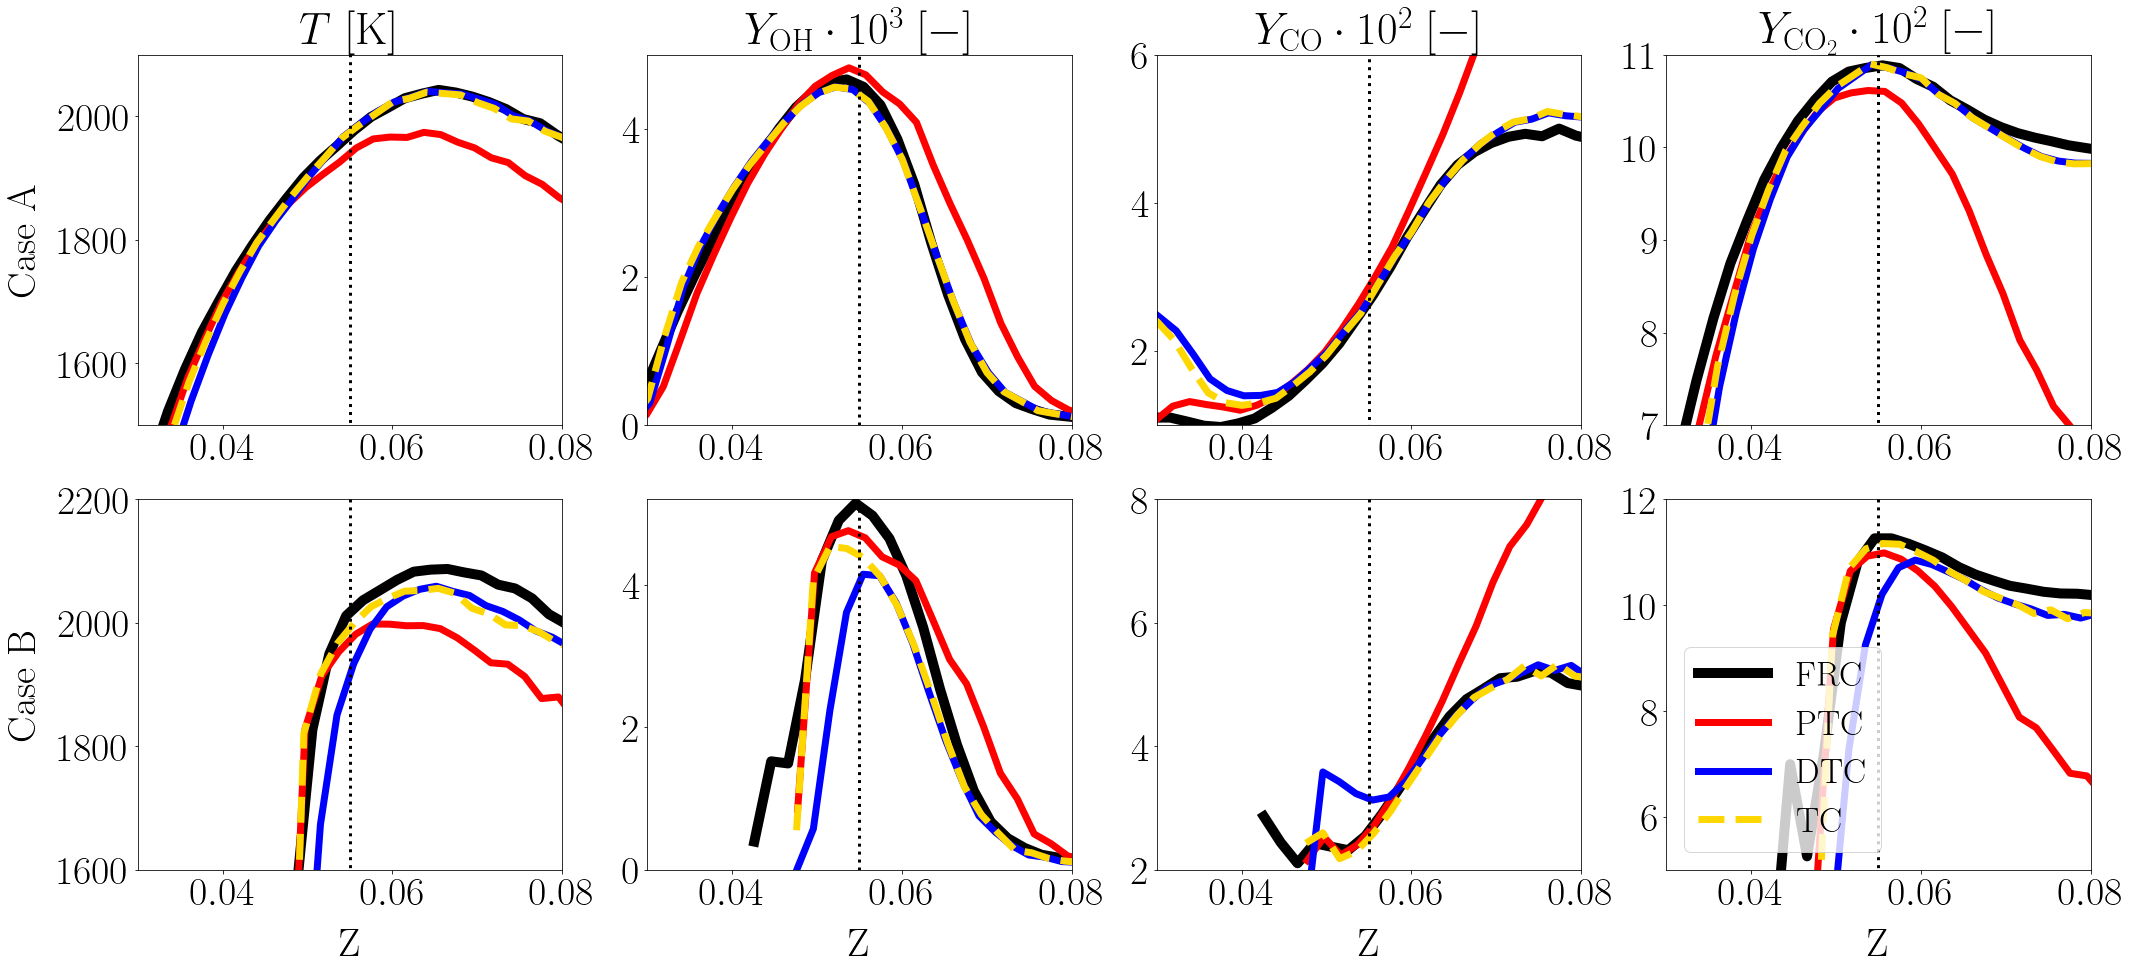
\includegraphics[scale=0.18]{./figures/fts_scatterplots_lines_A2}
    %\vspace{-0.5in}
	\caption{Conditional averages of temperature and mass fractions in the $Z$ space in area I for cases A and B. The vertical dotted line corresponds to $Z = Z_\mathrm{st}$.}
	\label{fig:fts_scatterplots_lines_A2}
\end{figure}


\begin{figure}[h!]
	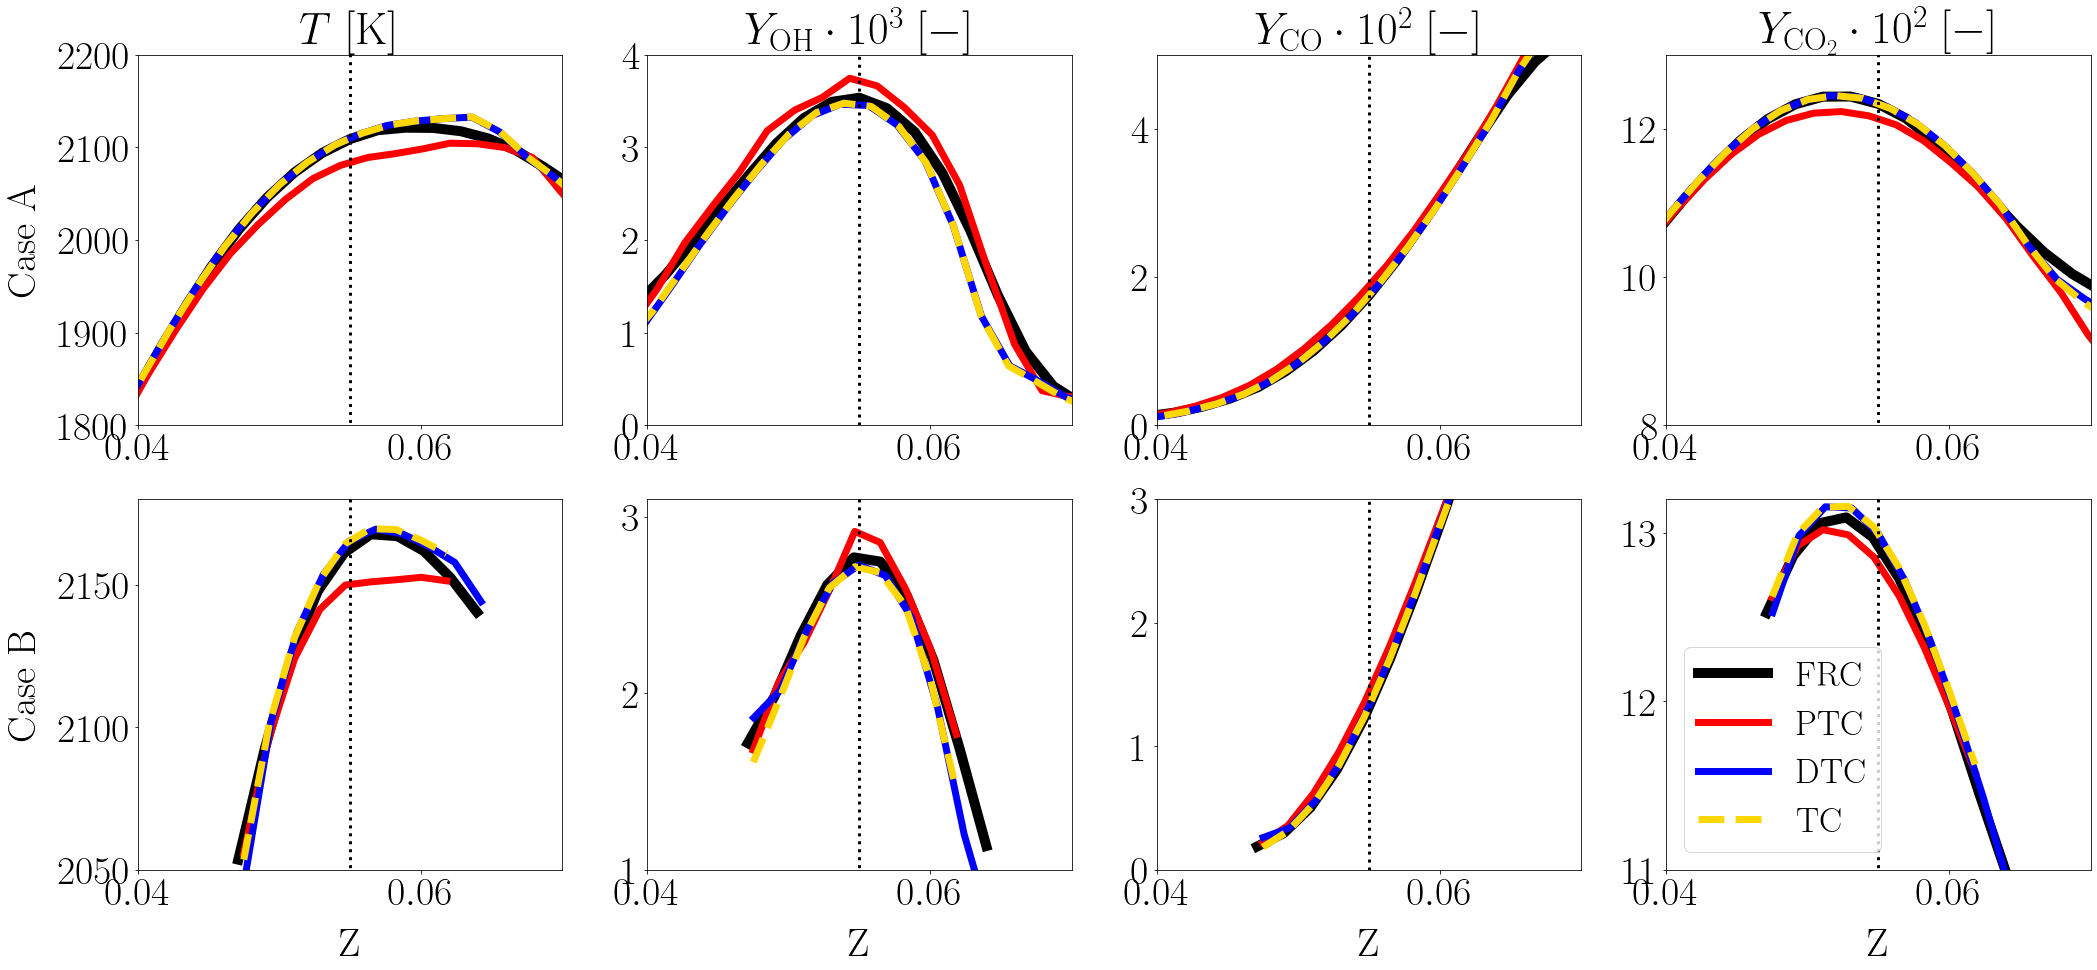
\includegraphics[scale=0.18]{./figures/fts_scatterplots_lines_A7}
    %\vspace{-0.5in}
	\caption{Conditional averages of temperature and mass fractions in the $Z$ space in area II for cases A and B. The vertical dotted line corresponds to $Z = Z_\mathrm{st}$.}
	\label{fig:fts_scatterplots_lines_A7}
\end{figure}

\dmm{\emph{WE SHOULD DISCUSS MORE IN DEPTH THIS RESULTS AND DISCUSS THE TRENDS OBSERVED IN THE RESULTS, WITH THE ABILITY OF THE INDEX TO REPRODUCE IT. WE SHOULD HIGHLIGHT HERE THE DISCREPANCIES OBSERVED FOR THE PREMIXED CASE THAT WERE NOT CLEAR IN PREVIOUS PLOTS. THIS IS KEY TO DEFEND THE USE OF OUR METHOD WITH RESPECT TO PREMIXED FLAMELETS}}



%TC computations with the multiregime model, using the premixedness index, have been run for all cases. Figure \ref{fig:fts_maps_comparison_flamelets} displayes the fields of temperature for all flamelet simulations (PTC, DTC, TC) and premixedness index $\xi_\mathrm{PF}$. 
%The $\xi_\mathrm{PF}$ distribution shows that all cases present regions of premixedness and diffusion. 
%Case 0, which corresponds to a diffusion jet, is mostly dominated by diffusion, which proves the capability of the index to identify this limit. 
%Premixedness levels then increase from cases A to D, where $\xi_\mathrm{PF}$ identifies mostly premixed combustion for the latter case except in a region around the centerline corresponding to a diffusion branch.

%Premixedness levels then increase from cases A to D, where in the latter $\xi_\mathrm{PF}$ identifies mostly premixed combustion except in a region around the centerline corresponding to a diffusion branch. This region is identified as non-premixed in all cases. 

%The temperature fields show that the multiregime computations recover values comprised between the premixed and diffusion flamelets, averaged according to the value of index $\xi_\mathrm{PF}$. Cases 0, A and B present the highest temperatures in the diffusion branch which matches the values and shape from the diffusion flamelet computation. Cases C shows higher temperatures in the lip between the central and outer injectors that match the diffusion case, while further radially the regimes corresponds to that of premixedness. In cases B and D, the most significant feature is the shape of the Bunsen flame, which in the multiregime computation retrieves the length of the premixed case, slightly shorter than the diffusion computation.




%\subsection{Learning model parameters from DNS}

%Working on this now (learning the k parameter and/or challenging the linearity hypothesis, for instance). 

\section{Conclusion}
\label{sec:conclusion}

In this paper, multiregime combustion in co-axial laminar flames has been simulated and analyzed. Computations have been carried out with a Direct Chemistry (DC) approach that solves the species transport equations, and also with a Tabulated Chemistry (TC) framework that combines premixed and diffusion flamelet tables using the premixedness flame index $\xi_\mathrm{PF}$ as weighting parameter. The DC computations illustrate the multiregime nature of the cases, which vary depending on the relative proportion of fuel with respect to air being introduced through the inlets. An a-priori analysis of DC computations showed that the index $\xi_\mathrm{PF}$ can detect premixed and diffusion regions similarly to the Takeno index, but with a more continuous variation among regimes. A-posteriori application of $\xi_\mathrm{PF}$ in TC computations shows the capability of this index to identify regimes and blend the table properties so that the results are closer to DC computations than when individual regimes are considered. Temperature and major species such as $OH$ and $CO_2$ are accurately predicted, while minor species such as $CO$ show larger discrepancies. Both Takeno index and $\xi_\mathrm{PF}$ \textbf{are unable to capture the nonpremixed mixing region downstream the injectors, which is known to be a challenging limit to be captured since the gradients of fuel and oxidizer are aligned as in a premixed flame} \citep{novoselov_two-dimensional_2021}. Continuing works should focus on accurately retrieving this limit, for example by using a non-linear progress variable that can intrinsecally identify the premixed and diffusion limits \citep{novoselov_two-dimensional_2021}, and to improve the prediction of minor species.

\textbf{The inability of this index to }


\appendix
\section{Comparison of $\xi_\mathrm{PF}$ application with and without $C$ threshold}
\label{sec:app_index_with_without_threshold}

The proposed modification of the premixedness index $\xi_\mathrm{PF}$ to recover the diffusion limit (Eq.~\textbf{XX}) is compared to the unmodified version (Eq.~\ref{eq:zeta_PF_illana}) applied in flamelet computations. In this appendix, results by applying the the original index is denoted as $\xi_\mathrm{PF}$ and the modified ones as $\xi_\mathrm{PF}^\mathrm{D}$. Fig.~\ref{fig:app:fts_maps_T_xi} shows the temperature and premixedness index fields. Differences between both types of computations are observed in the central region downstream the central injector. When the unmodified index is used in the computations, premixedness is detected and temperatures are lower than when the diffusion modification is considered, which identifies diffusion in this region. Contours of heat release rate $ \frac{\dot{\omega}_T }{\max \left( \dot{\omega}_T \right) } = 0.001$ are also shown in the $\xi_\mathrm{PF}$ field to illustrate that these modifications acts in the regions of low heat release rate. 

\begin{figure}[h!]
    \centering
	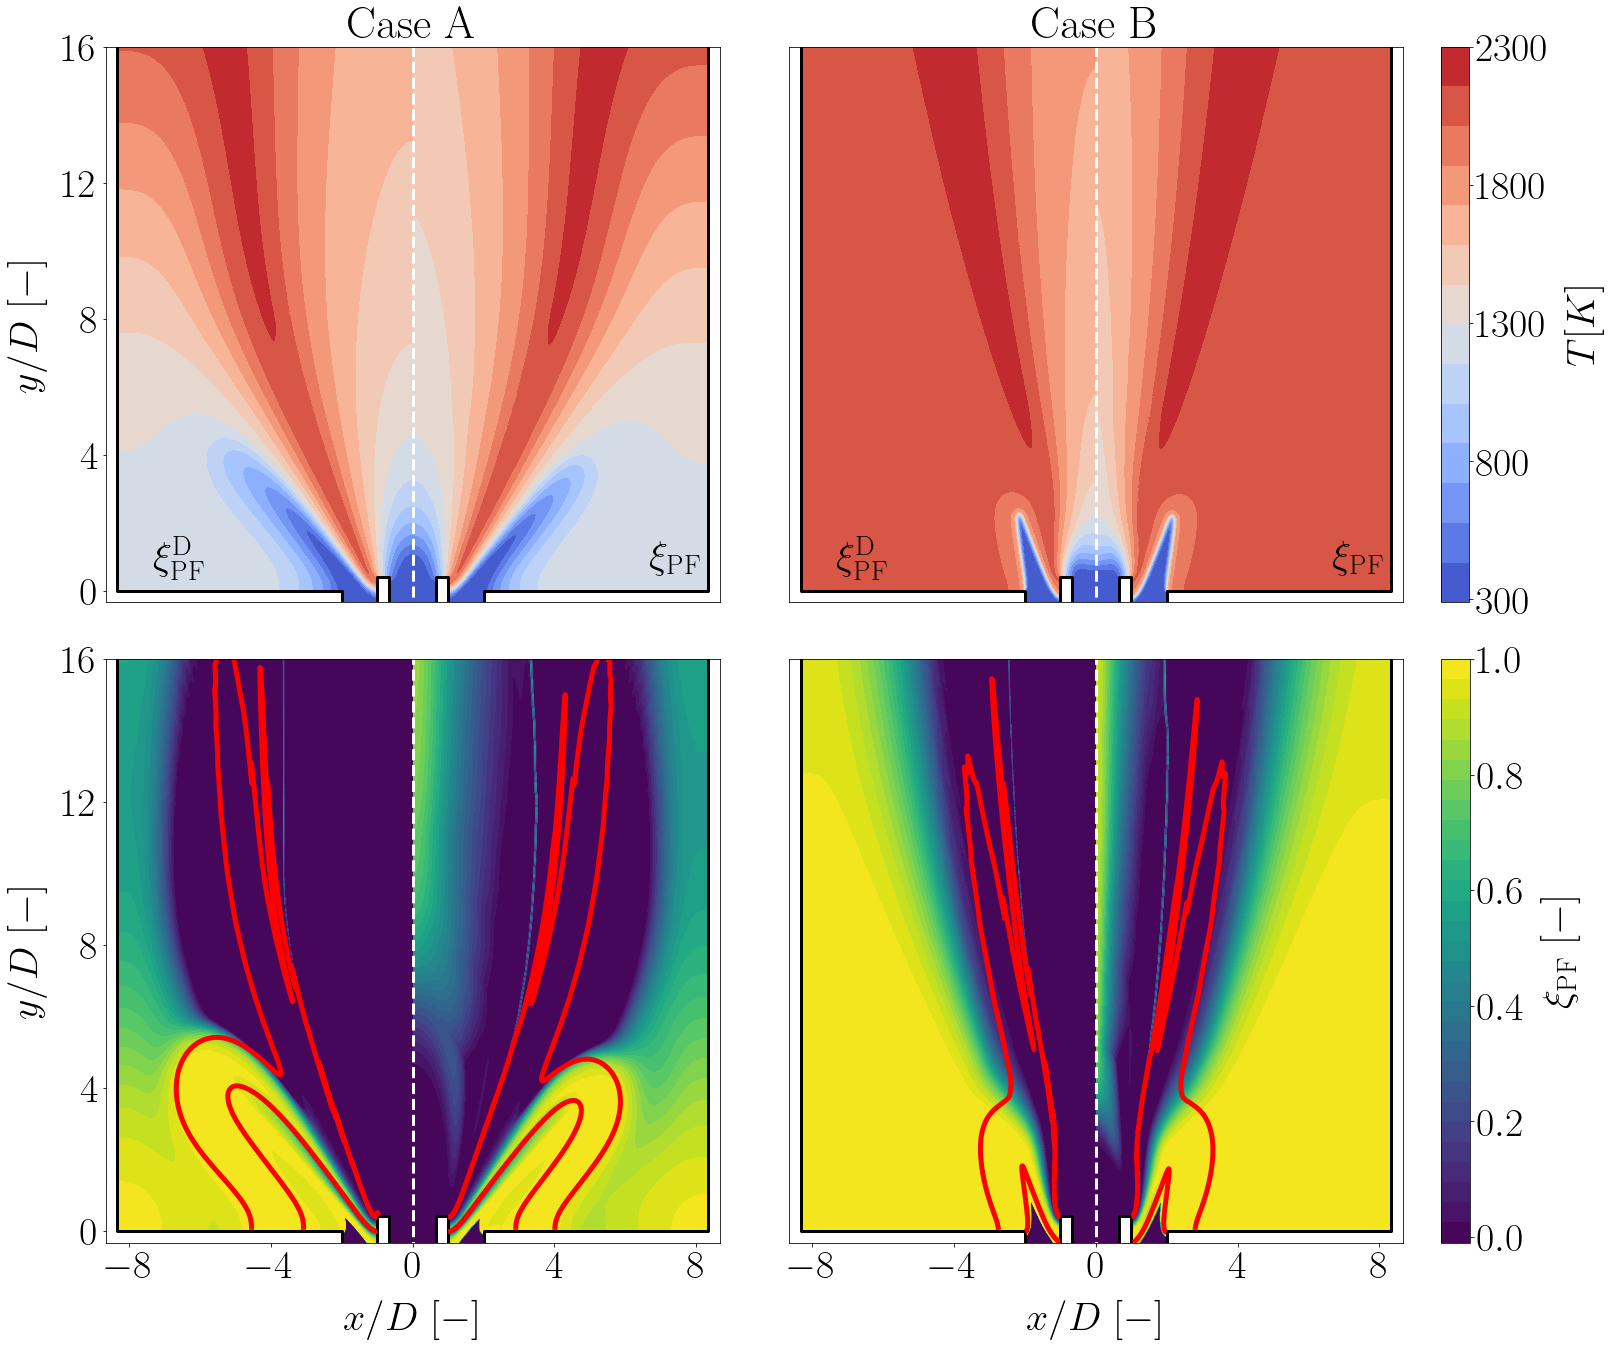
\includegraphics[scale=0.2]{./figures_appendix/fts_maps_T_xi}
    %\vspace{-0.5in}
	\caption{Temperature and premixedness index fields for flamelet simulations of cases A and B. The half-right side shows computations with the original index $\xi_\mathrm{PF}$, and the half-left side shows the modified index $\xi_\mathrm{PF}^\mathrm{D}$. The red contours in the index fields denote the contours of heat release rate $ \frac{\dot{\omega}_T }{\max \left( \dot{\omega}_T \right) } = 0.001$.}
	\label{fig:app:fts_maps_T_xi}
\end{figure}


To validate the modified index, the temperature profiles along the centerline $x = 0$ are shown in Figure \ref{fig:app:fts_profiles_T_line_x00}. Multiregime TC computations are compared against DC, DTC and PTC. The results show that computations using diffusion flamelets recover the values of DC, while premixed flamelets underestimate the temperature. Consequently, when the original index definition is used in a multiregime TC computation, temperature evolves initially following diffusion flamelets but quickly switches to follow the premixed line, underpredicting DC values. This is caused by the index evolving from $\xi_\mathrm{PF} = 0$ to $1$ since the mixture fraction enters into the flammability limits where the gradients of fuel and oxidizer are counter-aligned, as pointed out in Fig.~\ref{fig:flame_1D_flame_index}. Contrarily, when the modified index is considered, $\xi_\mathrm{PF}^\mathrm{D}$ stays at $0$, hence the multiregime TC computations account for diffusion in this region and temperature accurately follows the DC trends. 

\clearpage


\begin{figure}[h!]
    \centering
	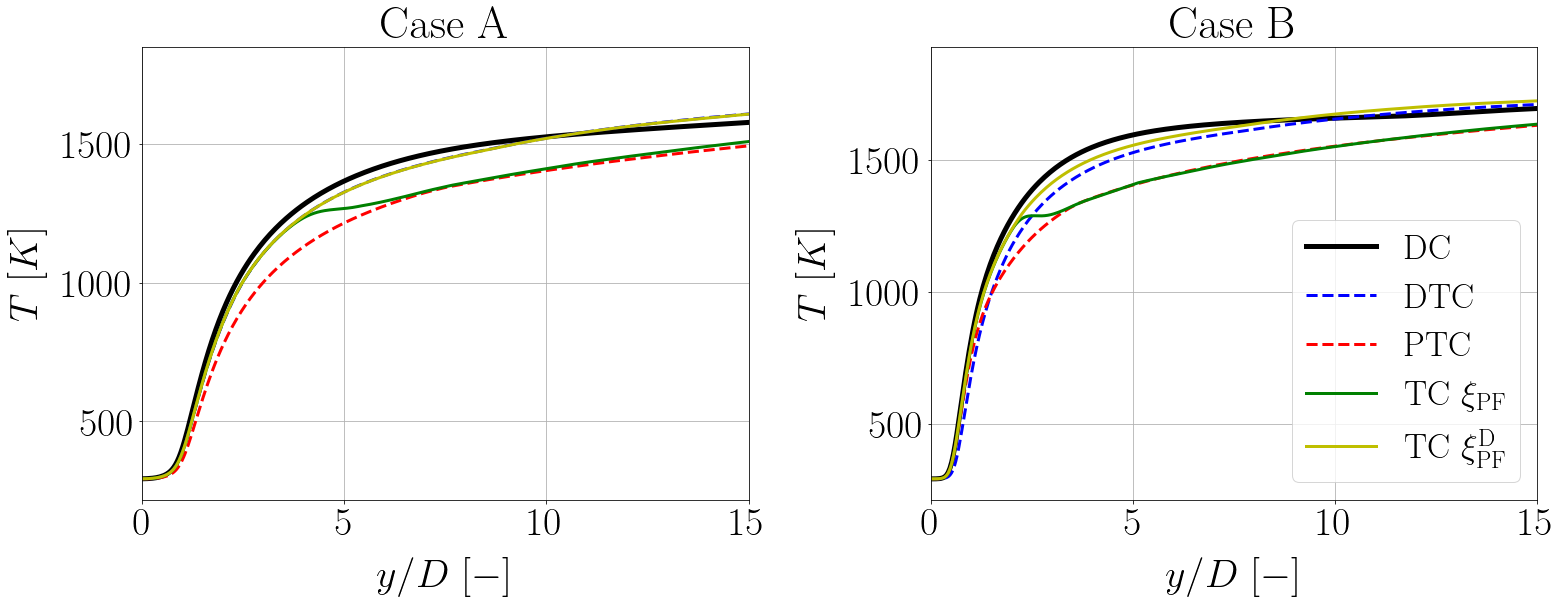
\includegraphics[scale=0.25]{./figures_appendix/fts_profiles_T_line_x00}
    %\vspace{-0.5in}
	\caption{Temperature profiles along the centerline $x = 0$ for Direct Chemistry (DC), diffusion (DTC) and premixed (PTC) tabulated chemistry, and multiregime tabulated chemistry with the original (TC $\xi_\mathrm{PF}$) and modified (TC $\xi_\mathrm{PF}^\mathrm{D}$) premixedness indices.}
	\label{fig:app:fts_profiles_T_line_x00}
\end{figure}






%\section*{Acknowledgements}
%\input{acknowledgements}


%% The Appendices part is started with the command \appendix;
%% appendix sections are then done as normal sections
%% \appendix

%% \section{}
%% \label{}

%% If you have bibdatabase file and want bibtex to generate the
%% bibitems, please use
%%
\bibliographystyle{elsarticle-harv} 
\bibliography{bibliography}

%% else use the following coding to input the bibitems directly in the
%% TeX file.

%\begin{thebibliography}{00}

%% \bibitem[Author(year)]{label}
%% Text of bibliographic item

%\bibitem[ ()]{}

%\end{thebibliography}
\end{document}

\endinput
%%
%% End of file `elsarticle-template-harv.tex'.
